\renewcommand\thisdir{papers/lcss22}
\tikzsetfigurename{lcss22-}
\renewcommand\figdir{\thisdir/figs}

% Commands for this paper
% if the conflict with previously defined commands use \renewcommand
%%%%%%%%%%%%%%%%%%%%%%%%%%%%%%%%%%%%%%%%%%%%%%%%%%%%%%%%%%%%%%%%%%%%%%%%%%%%%%%%
% In this file, only commands are allowed. These commands should be explained to
% greatest possible extent.
%%%%%%%%%%%%%%%%%%%%%%%%%%%%%%%%%%%%%%%%%%%%%%%%%%%%%%%%%%%%%%%%%%%%%%%%%%%%%%%%

% Real-time
\newcommand{\counter}{q}

% Plots
\newcommand{\timeplotheight}{4.9cm}

% Tables
\definecolor{Gray}{gray}{0.9}
\newcolumntype{a}{>{\centering\arraybackslash\columncolor{Gray}}m{0.075\columnwidth}}
\newcolumntype{b}{>{\centering\arraybackslash\columncolor{white}}m{0.075\columnwidth}}

% Set number of bins for aggregated plants histograms
\newcommand{\binsaggregatedhist}[0]{65}

%%% Colors
\definecolor{misscolour}{RGB}{255, 0, 0}
\definecolor{lqrcolour}{RGB}{0,28,255}
\definecolor{lqrnomcolour}{RGB}{0,28,255}
\definecolor{lqgcolour}{RGB}{0,139,0}
\definecolor{lqgnomcolour}{RGB}{0,139,0}
\definecolor{adacolour}{RGB}{239,133,16}


\paper[Stability under Extended Weakly-Hard Constraints]{Stability of Linear Control Systems under Extended Weakly-Hard Constraints}
\authors{Nils Vreman \and Paolo Pazzaglia \and Victor Magron \and Jie Wang \and Martina Maggio}

\begin{abstract}
    Control systems can show robustness to many events, like disturbances and model inaccuracies.
    It is natural to speculate that they are also robust to alterations of the control signal pattern, due to sporadic late completions (called \emph{deadline misses}) when implemented as a digital task on an embedded platform.
    Recent research analysed stability when imposing constraints on the maximum number of consecutive deadlines that can be missed.
    This is only one type of characterisation, and results in a pessimistic analysis when applied to more general cases.
    To overcome this limitation, this paper proposes a comprehensive stability analysis for control systems subject to a set of generic constraints, describing the possible sequences  of correct completions and deadline misses.
    The proposed analysis brings the assessment of control systems robustness to computational problems one step closer to the controller implementation.
\end{abstract}

\vfill
\textcolor{red}{This is an extended version of the paper} originally published in IEEE Control Systems Letters (2022). 
Reprinted with permission.
\newpage

\section{Introduction}
\label{sec:intro}
A recent survey on the state of industrial practice in real-time systems showed that a significant fraction of real-time tasks are allowed to miss a finite number of deadlines~\cite{Akesson:2020}.
%
The research community spent years defining and analysing models of tasks that can miss deadlines, from soft real-time systems~\cite{Buttazzo:2005}, to tasks with a skip-factor~\cite{Koren:1995}, from calculating the miss ratio based on execution time probability distributions~\cite{Manolache:2004}, to approximating the deadline miss probability~\cite{vonDerBruggen:2018, Bozhko:2021, vonderBrueggen:2021} for a given system.

One of such models in which tasks may miss deadlines is the weakly-hard task model~\cite{Bernat:2001}. 
Weakly-hard tasks behave according to patterns of hit and missed deadlines that are (mainly) window-based.
The originally proposed constraint models specifies alternatively (for a window of subsequent jobs):
\begin{enumerate*}[label=(\roman*)]
    \item the minimum number of deadlines that are hit,
    \item the minimum number of consecutive deadlines that are hit,
    \item the maximum number of deadlines that may be missed, or
    \item the maximum number of consecutive deadlines that may be missed.
\end{enumerate*}
The third of these models -- often called the $(m,K)$ model -- gained attention in the research community, generating results on scheduling algorithms~\cite{Hamdaoui:1995}, real-time and schedulability analysis~\cite{Sun:2017, Pazzaglia:2021b, Hammadeh:2017}, verification~\cite{Huang:2019b, Behrouzian:2020} and runtime monitoring~\cite{Wu:2020} of constraint satisfaction, derivation of task model parameters~\cite{Xu:2015}, together with applications to domains like telecommunication~\cite{Ahrendts:2018, Huang:2019a} and control systems~\cite{Ramanathan:1999, Pazzaglia:2018, Vreman:2021, Pazzaglia:2021}. 
The fourth model has also proved relevant to perform analyses of the stability of control systems~\cite{Maggio:2020}. 
Furthermore, the relation between weakly-hard constraint types has been partially investigated~\cite{Tu:2007, Wu:2020}.
However, this investigation remains partial as some of the constraints are not connected and their dominance (i.e., the comparison of how strictly does the task model constrain the task execution for different types of constraints) is not assessed.

The practical usefulness of weakly-hard models will remain limited, unless it is possible to build tools to enforce and monitor the satisfaction of weakly-hard constraints for execution platforms.
Many real-time platforms offer the possibility to invoke ``protected'' task executions, ensuring that deadlines are met at the cost of increasing the execution cost.
This is a very simple mechanism to secure that the weakly-hard constraint is satisfied in an execution platform.
However, this requires writing monitoring code, that generates transition points to this protected execution mode when a constraint might otherwise be violated.
Generating this code in a scalable way requires abstracting from the constraint and representing the execution of tasks with compact, but expressive, models.

To date, the literature has focused on the $(m,K)$ constraint, neglecting the others, despite their relevance in application domains such as control~\cite{Maggio:2020, Linsenmayer:2017, Vreman:2021}.
As a result, the mentioned tools and models are not available for all the constraint types.
This paper aims at both solving this problem and answering some open issues, namely:
\begin{enumerate*}[label=(\roman*)]
    \item guaranteeing consecutive deadline hits, and not only following patterns of deadline misses; and
    \item dealing with systems that satisfy multiple weakly-hard constraint simultaneously.
\end{enumerate*}

The first issue comes from the consideration that in practice it may be easier to guarantee that some prescribed job will hit their deadline rather than ensuring that the number of misses follows a given pattern. 
This is the case of the mentioned protected execution environment. 
As an example, mixed-criticality allows the scheduler to raise the criticality level and thus guarantee that the highly-critical tasks meet the corresponding deadlines~\cite{Burns:2013}. 
We can treat the weakly-hard task as highly critical and raise the criticality level when a deadline hit must be enforced. 
Alternatively, we can increase the budget of a reservation-based scheduler~\cite{Casini:2019}.
Despite the fact that guaranteeing hits is often easier than enforcing miss patterns, the first two types of weakly hard tasks, that constrain the number of hits, have not been receiving much attention from the research community.

Furthermore, we would like to analyse tasks that satisfy multiple constraints simultaneously.
Most analysis methods only take into account a single constraint, e.g.,~\cite{Pazzaglia:2018} or~\cite{Maggio:2020} for the stability of control systems.
In some cases, one of the two constraints \emph{dominates} the other, meaning that satisfying the dominant constraint also guarantees the satisfaction of the dominated one. 
But this is not always the case.
Consider for example two constraints $\lambda_1$ and $\lambda_2$, where $\lambda_1$ specifies that the task may miss a maximum of 2 deadlines in every window of 5 consecutive jobs, and $\lambda_2$ that it may miss a maximum of 3 deadlines in every window of 7 consecutive jobs.
On the one hand the sequence 0011100, where 0 represents a deadline miss and 1, satisfies $\lambda_1$ but fails $\lambda_2$, meaning that $\lambda_2$ does not dominate $\lambda_1$.
On the other hand the sequence 0001111 satisfies $\lambda_2$ but fails $\lambda_1$, and so $\lambda_1$ does not dominate $\lambda_2$ either.
If the analysis can only be conducted with a single constraint, the choice of which constraint is to be used is left to the practitioner, while it would be best to consider \emph{both} constraints simultaneously.

Finally, we bring forward the question of \emph{scalability}. 
Many of the research results, for example in the control domain~\cite{Pazzaglia:2018, Linsenmayer:2017, Linsenmayer:2021}, use short windows. 
However, for practical applications it may be relevant to use a large window size, as done for example in the experimental analysis in~\cite{Behrouzian:2020}. 
In fact, the original motivation behind the weakly-hard task model~\cite{Bernat:2001} uses a practical example from the avionics domain in which a deadline may be missed $11$ times in every consecutive $295$ jobs. 
It seems reasonable that systems that are built and certified (for example in the automotive domain) would not experience many deadline misses, and that using a short window size would lead to very conservative results.

To address these questions and empower researchers with a tool to apply their analysis techniques, this paper presents \tool, a software library for weakly hard tasks that treats scalability as a first-class citizen. 
More precisely, the contributions of the paper are the following:

\begin{itemize}

    \item We provide a theoretical contribution on the relation between weakly hard tasks that constrain the number of hits and the number of consecutive hits in a window (Section~\ref{sec:theorems}). 
        This relation allows us to relate all the types of constraints with one another, and provide some ordering among them. 

    \item We leverage an automata-based representation to describe the behaviour of a task subject to a weakly-hard constraint~\cite{Horssen:2016, Linsenmayer:2021}.
        In constrast to other approaches, our description exploits a mapping between a single transition in the automaton and a deadline (Section~\ref{sec:code}).
        This enables uses such as automatic generation of monitors to check weakly-hard constraint satisfaction on the fly.

    \item We extend the automaton to describe a task subject to a finite set of weakly-hard constraints (Section~\ref{sec:theorems}).
        In this way, we are able to address the analysis of systems that satisfy multiple constraints, possibly of different types, that do not dominate one another.
        As far as we know, this is the first paper that presents an analysis of a set of weakly-hard constraints.

\end{itemize}

We conduct an extensive performance evaluation campaign with a two-fold purpose (Section~\ref{sec:experiment}). 
First, we analyse the scalability of our library compared to the state of the art whenever possible, i.e., for single constraints. 
Second, we look at sets of constraints and perform a sensitivity analysis, to determine which parameters affect the execution time of the automaton construction for a set of constraints. 

\tool{} can be used for monitoring tasks subject to multiple weakly-hard constraints, analysing satisfaction sets, schedulability analysis, or connecting the weakly-hard model to applied fields like control theory.
In particular, recent papers~\cite{Pazzaglia:2018, Maggio:2020, Vreman:2021, Linsenmayer:2021, Linsenmayer:2017} connected the weakly-hard model with control proofs considering stability and performance guarantees, and \tool{} can generate general automata-based monitoring code ensuring the satisfaction of said properties.


\section{Background and Notation}
\label{sec:background}
\chapter{Background}%
\label{ch:background}%

This chapter presents the necessary background and motivation for the remainder of the thesis.
We divide the chapter in two primary parts.
First, a discussion on the real-time theoretical aspects is provided.
An extended introduction to how real-time operating systems operates is presented, e.g., processor sharing, task states, scheduling strategies, etc.
However, the main focus is dedicated to the most commonly used task models and their respective advantages and disadvantages, with respect to deadline overruns.
Additionally, we provide a brief discussion on state-machine applicability to the aforementioned task models. 
Next, the relevant control theoretical background is presented based on the theory of real-time systems.
Two different system modelling approaches are introduced: switching systems and Markov jump linear systems.
Both models are particularly relevant for real-time systems where the control task can overrun its deadlines.
Specifically for these systems, we present and discuss different stability and performance analyses.

\section{Real-Time Systems}%
\label{sec:background:rts}%
%
% A short extension to the RTS (and RTOS) precise objective
We begin with an introduction to real-time system fundamentals. 
The breadth of the topic prevents a comprehensive review of the existing literature to fit within the scope of this thesis.
In fact, real-time systems are all information processing systems which reacts to external input within a predetermined deadline. 
This includes sensors, actuators, process control, machine vision, robotics, and health care systems, to acknowledge a fraction of all real-time systems.
Instead, we focus the attention to the elements which impact real-time control systems the most, i.e., CPU provisioning, memory management, periodic tasks, task models, scheduling policies, and execution models.
Since the RTOS is tightly interconnected with the hardware, it is natural to illustrate them jointly.
Next, we describe the underlying hardware and real-time architecture seen in Figure~\ref{fig:operating-system-abstraction}.
%
\begin{figure}[t]
    \centering
    \def \delta {0.15}

\begin{tikzpicture}
\tikzstyle{task} = [draw,thick,fill=white,align=center]
\tikzstyle{circleconn} = [draw, fill=white, thick, circle, scale=0.5]

%%% TASKS %%%

\begin{scope}[on background layer]
    \node[task,opacity=0.3] (t1) at (-1.5+0*\delta,1.6-0*\delta) {\textcolor{white}{Task $\#3$} \\\textcolor{white}{\faFileCode[regular]}};
    \node[task,opacity=0.6] (t2) at (-1.5+1*\delta,1.6-1*\delta) {\textcolor{white}{Task $\#2$} \\\textcolor{white}{\faFileCode[regular]}};
    \node[task,opacity=1.0] (t3) at (-1.5+2*\delta,1.6-2*\delta) {Task $\#1$ \\\faFileCode[regular]};

    \node[task,opacity=0.3] (ct1) at (1+0*\delta,1.6-0*\delta) {\textcolor{white}{Control Task $\#3$} \\\textcolor{white}{\faFileCode[regular]}};
    \node[task,opacity=0.6] (ct2) at (1+1*\delta,1.6-1*\delta) {\textcolor{white}{Control Task $\#2$} \\\textcolor{white}{\faFileCode[regular]}};
    \node[task,opacity=1.0] (ct3) at (1+2*\delta,1.6-2*\delta) {Control Task $\#1$ \\\faFileCode[regular]};

    %%% CYBER %%%

    \node[thick, align=center] (rtos) at (-0.1,0.25) {Real-Time Operating System};
    \node[thick, draw, align=center, rotate=90, text width=2.75cm] (hwi) at (3.15,0.87) {HW Interfaces};
    \node[thick, fit=(rtos)(t1)(ct1)(ct3),draw,yshift=1.5mm,xshift=0.75mm] (sw) {};
    \node[thick, draw, above left] (clock) at (sw.south east) {\faClock[regular]};
    \node[thick, fit=(sw)(hwi), inner sep=7pt, draw] (hw) {};
    \node[thick, above left, xshift=2.3cm, yshift=0.5mm] (hw-label) at (hw.south west) {Hardware};
    \node[thick, draw, above right] (hwclock) at (hw.south west)  {\faClock[regular]};

    %%% PHYSICAL %%%

    \node[thick, draw ,align=center] (phys) at (6,0.87) {
\includegraphics[scale=4]{\figdir/airplane.jpg}};
    \node[thick, draw, above left] (time) at (phys.south east) {\faClock[regular]};
\end{scope}


%%% ZOOM %%%

% Tasks
\node[task] (vt1) at (-0.9+0*10*\delta,1.0) {Task $\#1$ \\\faFileCode[regular]};
\node[task] (vt2) at (-0.9+1*10*\delta,1.0) {Task $\#2$ \\\faFileCode[regular]};
\node[]           at (-0.9+2*10*\delta,1.0) {$\cdots$};
\node[task] (vtn) at (-0.9+3*10*\delta,1.0) {Task $\#N$ \\\faFileCode[regular]};

\node[circleconn] (c1) at ($(vt1)+(0,-0.75)$) {};
\draw[thick] (c1.north) to (vt1.south);
\node[circleconn] (c2) at ($(vt2)+(0,-0.75)$) {};
\draw[thick] (c2.north) to (vt2.south);
\node[circleconn] (cn) at ($(vtn)+(0,-0.75)$) {};
\draw[thick] (cn.north) to (vtn.south);

% CPU
\node[task, minimum width=1.3cm, minimum height=1.0cm] (cpu) at (-0.9+1.5*10*\delta,-2.25) {CPU};

% Memory
\node[thick, draw, align=center, rotate=90, text width=2.25cm] (mem) at (-1.0+4*10*\delta,0.1) {Memory};

% HW interfaces
\node[thick, draw, align=center, rotate=90, text width=0.8cm] (gpio) at (-1.0+4*10*\delta,-2.15) {GPIO};

% Background 

\begin{scope}[on background layer]
    \node[thick, dashed, fill=white, fit=(vt1)(vtn)(cpu)(mem),draw,inner sep=4pt] (vhw) {};
    \draw[thick, dashed] ([yshift=-0.85cm]vhw.west) to ([yshift=-0.85cm]vhw.east);
    \draw[thick, dashed] ([xshift=2.65cm]vhw.south) to ([xshift=2.65cm]vhw.north);
\end{scope}

\draw[thick, dashed] (hw.south west) to (vhw.south west);
\draw[thick, dashed] (hw.north west) to (vhw.north west);
\draw[thick, dashed] (hw.north east) to (vhw.north east);

% Scheduler
\node[task, minimum width=5cm] (sched) at (-0.9+1.5*10*\delta,-1.0) {Scheduler};
\node[circleconn] (csched) at ($(sched)+(0,0.5)$) {};
\draw[thick] (csched.south) to (sched.north);

\draw[thick, -latex] (csched.north) to (c2.south);
\draw[thick, dashed, -latex, opacity=0.3] (csched.north) to (c1.south);
\draw[thick, dashed, -latex, opacity=0.3] (csched.north) to (cn.south);


\end{tikzpicture}
%
    \caption{\fix{Need to arrange figure so it makes more sense.}}%
    \label{fig:operating-system-abstraction}%
\end{figure}

% CPU and cores
The \emph{central processing unit} (CPU, or simply \emph{processor}) is the electronic component responsible for executing the task functions.
Each function (or program) is translated into a list of instructions to be executed on the CPU.
These instructions belong to the machine's language used to tell the processor what type of operation to execute, e.g., load a specific memory register or execute an arithmetic operation.
The time it takes for the CPU to execute one instruction, i.e., fetching the instruction from memory before decoding and executing it, is typically called an \emph{instruction cycle} (or simply \emph{cycle}); this is the basic unit used to measure CPU speed.
To execute the program instructions, the processor can contain one or more \emph{cores}, respectively denoting the processor as \emph{single-core} or \emph{multi-core}.
Each core is able to execute a list of program instructions.
Hence, the advantage of using multi-core processors (compared to single-core processors) is the increased number of instructions that can be executed in parallel. 
However, this gain comes at the cost of an elevated system complexity where the memory and application layout has to be adapted to the multi-core architecture~\cite{Brandenburg:2011}.

% Memory
Integrated with the processor is a \emph{cache} memory, i.e., a small but fast memory that is easy to access from the operational cores.
The cache memory stores recently accessed instructions and data to reduce the latency induced by fetching from \emph{main memory}, i.e., the main hardware storage.
Most modern CPUs have a layered cache memory hierarchy, where the smallest and fastest layer is denoted L1, the second smallest and fastest is denoted L2, and so on.
When the processor needs to access some data, it first examines whether the data exists in the cache and in that case fetch it from there; otherwise, it collects the data from the main memory.

If a task wants to access cached data (or instructions) that cannot be found, it is said to experience a \emph{cache miss}; similarly, a \emph{cache hit} occurs when the sought data is found in the cache.
Cache misses can arise if:
%
\begin{itemize}
    \item the size of the requested data is too large to fetch;
    \item the requested data is not yet loaded into the cache; or
    \item the data have been evicted from the cache, e.g., to make room for more recently retrieved data or from the cache being flushed due to security reasons.
\end{itemize}
%
Ideally, the number of cache misses that a task experiences are kept to a minimum, in particular since fetching data from the main memory can incur large timing overheads on the task execution.
Additionally, the longer a task executes, the less likely it is to contract cache misses.
Intuitively, the task will experience a few initial cache misses when the data is loaded into the cache, but thereafter the cache will be occupied by relevant data and the cache misses should decrease.
This is also known as \emph{cache warming}.
If the task continues to experience significant cache misses even after the cache warming phase, it is said to be \emph{thrashing} the cache, i.e., continuously experiencing cache misses.
Thrashing can severely impact both real-time performance, energy consumption, and even collapse the execution~\cite{Wadleigh:2000}.
In multi-core setups where different cores share a level-X cache, thrashing is a big concern; however, there exists strategies to mitigate frequent interference from different tasks sharing the same cache~\cite{Brandenburg:2011}.
To help mitigate cache eviction (both in single- and multi-core setups), \emph{cache partitioning} is typically employed.
Cache partitioning reserves specific memory addresses for specific tasks, whilst reserving others for shared data.
Thus, cache evictions are limited to the specific cache memory regions that are shared among multiple tasks; unless, the cache is flushed due to security reasons.

% GPIO 
To interface with the external environment, the hardware uses \emph{input/output peripherals} (I/O peripherals).
The peripherals are all external components connected to the hardware, e.g., sensors, actuators, or routers.
Depending on the hardware, the peripherals can either be connected to the circuit board responsible for joining the different components together or directly into the CPU.
If the link to the external environment is wireless, the I/O peripherals are not necessarily sensors or actuators, but rather radio antennas, Bluetooth transmitters, or Wi-Fi routers (depending on the wireless communication protocol) interacting with the sensors and actuators.
Typically, each peripheral is assigned to an \emph{I/O port} in the device, i.e., a unique number to know which physical pin to transmit and receive data through. 

% Microcontrollers and embedded systems
\nv{Not sure if this paragraph should be higher up (in connection to the I/O), or not?}
Although this thesis does not discern different hardware architectures from one another, it is appropriate to talk about \emph{microcontrollers} and \emph{embedded systems}, in particular because of their growing recognition. 
Despite being two different hardware architectures, the terms embedded system and microcontroller will carelessly be used interchangeably due to their natural similarities.
As introduced in Chapter~\ref{ch:intro}, microcontrollers (MCUs) are small computers with integrated processors, memory, and I/O peripherals.
Most embedded systems are based on microcontroller architectures, however, some embedded systems are based on one or more microprocessors with external memory and I/O peripherals.
Hence, microcontrollers are embedded systems and can be used to develop more complex embedded systems, but an embedded system is not necessarily a microcontroller.
\nv{Not sure if this paragraph should be higher up (in connection to the I/O), or not?}


Separately from the I/O port, the \emph{communication protocol} defines the rules used to pack and unpack the packets sent between the peripherals and the hardware over the \emph{communication channel}.
As an analogy, consider a postcard being sent between England and France; the port is where we choose to send the letter, i.e., the address to send it to and the postage stamp, while the protocol is the content of the message, i.e., the chosen communication format.
Communication protocols and their implementation details belong to a vast research topic which falls outside the scope of this thesis.
However, it is an important component of real-time networked control systems and is thus briefly introduced here.

% More into depth about the communication channel and what problems we might encounter here
Information transmitted over a network (wired or wireless) is generally represented as a set of bits (ones and zeroes) to be read in series or parallel; without loss of generality, we will only mention the serial case.
The communication protocol defines the rules determining how the transmitter should encode its data in order for the receiver to decode it using the same set of rules.
The rules are highly dependent on the communication protocol and its application domain.
We illustrate the idea of communication protocols with an example: consider the case where a transmitter wants to send the character \code{R} using the universal asynchronous receiver-transmitter (UART) protocol\footnote{Assuming ASCII encoding of the character, 8 data bits, no parity, and 1 stop bit, i.e., UART 8-N-1.}.
The rules defined by this protocol states that each data packet contains exactly 8 bits of information, is prepended with a start bit ($0$), and is appended with a stop bit ($1$).
Since the binary representation of \code{R} is $01010010$ (using ASCII encoding), the encoded character's packet representation to be sent over the network is then:
%
\begin{equation*}
    \underbracket{0}_{\text{Start bit}} \;\, \underbracket{01010010}_{\text{Data bits}} \;\, \underbracket{1}_{\text{End bit}}.
\end{equation*}
%
Transmitting a message, such as \code{RTS}, thus involve encoding each character individually before transmitting the encoded bit stream in sequence:
%
\begin{equation*}
    0\underbracket{01010010}_{\code{R}}1 \;\;
    0\underbracket{01010100}_{\code{T}}1 \;\;
    0\underbracket{01010011}_{\code{S}}1.
\end{equation*}

The network over which the packets are transmitted, typically consist of one or more routers forwarding the packets between different target locations.
To determine where to forward the packet to, the packet includes a \emph{network address}\footnote{The network address is an identifier to help recognise where to froward the packet to. Common examples of network addresses are IP addresses and MAC addresses.} that is read by the router before rerouting the packet according to a routing policy.
Additionally, each router contains a buffer to store incoming packets before processing them.
Processing the packets in the buffer is efficient, but it requires some non-negligible overhead, i.e., reading the network address and deciding where to forward the packet.
Thus, under normal conditions the receiver will experience packet latency and jitter, but if the network traffic is heavy the buffer space can quickly be exhausted.
In other words, if the packets arrive faster than what the router can process it becomes congested.

Multiple policies have been developed to control the congestion, e.g., tail drop~\addref{} and \nv{insert something}~\addref{}.
Common among all the congestion control strategies is that they employ intentional \emph{packet dropping}, i.e., if a packet arrives while the buffer space is exhausted, the congestion controller will remove either the arriving packet or one in the buffer (depending on the strategy).
In addition to the congestion controller dropping packets, there are intermittent packet drops due to, e.g., packets being misrouted~\addref{}, security threats~\addref{}, software bugs~\addref{}, or wireless communication~\addref{}.

Regardless of the packet drops' origins, they can have dire consequences for real-time control systems.
Losing packets on the network connecting the control hardware and the plant, is the same as loosing sensor measurements or control commands.
Generally, this will degrade the control performance~\addref{}, however, if enough packets are lost it could cause critical system failures or crashes~\addref{}.

% RTOS, threads
A real-time operating system is commonly employed to simplify the interface with the hardware while guaranteeing timeliness.
The RTOS is responsible for orchestrating the tasks' execution and allocating resources (e.g., memory and CPU time) to said tasks.
The terms ``task'', ``process'', and ``thread'' are frequently confused in many documents; to avoid this confusion we provide a definition in the context of real-time operating systems~\addref{}:
%
\begin{itemize}
    \item \emph{Process} -- A process is a computer program with its own stack, control block\footnote{A task's control block (TCB) includes descriptive information about the task, for instance, the identifier used by the scheduler, its priority, and the task's state (running, ready, blocked, suspended, etc.).}, and instruction set.

    \item \emph{Thread} -- A thread is an entity within a process that share the memory context with additional threads.

    \item \emph{Task} -- The term \emph{task} is used analogously with \emph{process}.
\end{itemize}
%
The notational confusion likely arose from the \emph{multithreading}, \emph{multiprocessing}, and \emph{multitasking} paradigms.
In a multiprocessing environment, multiple tasks can execute concurrently, each on a separate core; multithreading is a CPU feature for executing multiple threads concurrently on a single core; and, multitasking is when a single core is executing multiple tasks concurrently.

% Scheduler (how it allocates resources), threads, mechanisms, ISR
The RTOS typically employ a scheduler to orchestrate the tasks and to provide them with the appropriate resources.
The scheduler is responsible for switching tasks in and out, making sure that the correct task context (the task's resources) is brought into scope, handling interrupts, and ensuring fairness among the entities sharing the resources, e.g., interrupts, tasks, and kernel methods.
How the scheduler assigns resources is decided by the \emph{scheduling algorithm}.
Most scheduling algorithms adopt a \emph{preemptive} approach to assigning resources, i.e., the scheduler is run once every time slice (time quanta) to choose which task to switch in.
Classical examples of preemptive scheduling algorithms are:
%
\begin{enumerate*}[label=(\roman*)]
    \item fixed priority preemptive (FPP), where the task with the highest predetermined priority value is executed;
    \item earliest deadline first (EDF), where the task with the shortest time to its corresponding deadline is executed; and
    \item round-robin (RR), where the tasks are switched into scope in a circular order.
\end{enumerate*}
%
Depending on the choice of algorithm, the real-time system's execution pattern may vastly differ.
For instance, two different scheduling strategies applied to one set of real-time tasks, may or may not result in the system being \emph{schedulable}, i.e., all the temporal constraints are satisfied.
If the RTOS tasks are not schedulable there exists tasks overrunning their corresponding deadlines.

In order for the scheduler to know when to stop the currently running task in favour of switching in another, the RTOS clock triggers an \emph{interrupt} at every clock tick.
Interrupts can come from both hardware\footnote{Hardware interrupts come from events changing the state of the system, e.g., external signals triggering that they need attention from the RTOS, watchdog timers triggering an interrupt at set time intervals, or spurious interrupts (electrical anomalies)~\addref{}.} and software, but the RTOS ticks are triggered by the software clock in the RTOS.
Attached to the interrupt is generally an \emph{interrupt service routine} (ISR), i.e., a callback function to execute when the specific interrupt is triggered.
For instance, in the context of the scheduler's tick interrupt, the ISR may be responsible for switching out the currently active task before switching in a new task and its relevant context.
The ISR connected to the RTOS clock tick is also one of the major culprits behind \emph{release jitter} in RTOS, i.e., the time it takes to put the suspended task into the ready queue before picking a new candidate to execute varies between invocations.
Since the RTOS suspends the execution of the active task whenever an interrupt is triggered (even if it happens in the middle of a time slice), it is crucial that the ISR is quick to execute to avoid stalling the processor.
Hence, if the callback function takes too long to execute or if the ISR is triggered too often, it can cause significant time delays in the schedule execution.

Employing a scheduler for single-core processors follow the described paradigm, however, for multi-core systems additional design choices have to be made.
Fundamentally, two different approaches have been taken to scheduling to a multi-core processor: \emph{global} or \emph{partitioned} scheduling.
The former assumes one scheduler responsible for scheduling all the tasks in a global ready queue to the individual cores based on available and required resources.
On the other hand, partitioned scheduling (sometimes referred to as \emph{clustered} scheduling) involves dividing the tasks into partitions that are then mapped to separate cores with individual schedulers.
Despite having additional computational resources to work with, multi-core systems are subject to deadline overruns similarly to how single-core systems are.
Trivially, since partitioned multi-core scheduled systems can be perceived as a set of single-core scheduled systems, they can also experience the same computational overruns that a single-core system can.
For global multi-core schedulers, \nv{I need some help completing this sentence, I got lost in pfair schedulers and got confused}
\fix{Concluding sentence that confirms that this thesis is relevant even for multi-core systems.}


\subsubsection*{\note{Tasks}}%
% Tasks
All the real-time tasks considered in this thesis are \emph{recurrent}, i.e., they do not terminate during system operation.
The recurrent task model simplifies the \emph{a priori} analysis of the real-time workload's effect on the system execution.
A plethora of methods have been derived to model the recurrent task execution, ranging in complexity from the classic Liu and Layland model~\cite{Liu:1973} to directed acyclic graph (DAG) models~\cite{Saifullah:2014}.
Henceforth, the terms \emph{recurrent tasks} and \emph{tasks} will be used analogously.

The task model adopted in this thesis defines a task $\tau$ as a sequence of \emph{jobs} $j_t$, where each job is responsible for executing one full iteration of the task's function.
Here, $t$ counts the number of discrete time steps since the task was created.
Each task $\tau_i$ is characterised by the triplet $(e_i, d_i, p_i)$.
Here, for each job; $e_i > 0$ is the \emph{worst-case execution time} (WCET); $d_i > 0$ is the relative \emph{deadline}; and, $p_i \geq d_i$ is the minimum interarrival \emph{period}.
The RTOS scheduler releases a job $j_t$ at time $a_t$ (the job's \emph{release time}) and the job then completes its execution at time $f_t$ (the job's \emph{completion time}).
A recurrent task is \emph{periodic} if its jobs are released at equidistant time points, i.e., $a_t = t\cdot T$ where $T$ is fixed. 
In particular, control tasks are typically implemented as periodic tasks, hence one job is released in every period.
To make sure that the periodic task's jobs finish their execution before the subsequent job is released, it is common to adopt \emph{implicit deadlines}, i.e., that job $j_t$ completes its execution before the release time of job $j_{t+1}$; formally, it implies that $f_t \leq a_{t+1} = t\cdot T+T = a_t + T$ or simpler $d_i = p_i = T$.

Under ideal computational conditions, each job completes its execution before its corresponding deadline, i.e., $f_t \leq a_t + d_i$.
However, it can happen that the individual job has not yet finished executing when it reaches the end of its allotted time budget.
We then say that the job experiences a \emph{deadline overrun} (also referred to as \emph{deadline miss} or \emph{computational overrun}).
Respectively, if the job completes before its deadline, it \emph{meets} its deadline (experiences a \emph{deadline hit}).
%
\begin{definition}[Deadline Overrun]%
    \label{def:kappa:overrun}%
    The $t$-th job ($j_t$) of a task $\tau_i$ is said to experience a deadline overrun if
    \begin{equation}
        f_t > a_t + d_i.
    \end{equation}
\end{definition}
%
Computational overruns are present in generally all real-time domains from avionics and defence to consumer electronics~\cite{Akesson:2020}, thus highlighting the importance of analysing their impact on the systems' functional correctness.

% task models -> soft, hard, weakly-hard
Every real-time systems behave differently to deadline overruns.
Depending on the application, some systems crash while others experience a degraded efficiency.
Due to this individuality, most real-time systems were historically divided into two classes describing how the systems were affected by computational overruns.
%
\begin{itemize}
    \item \emph{Hard real-time systems} -- It is imperative that the deadlines are met in order to prevent critical system failure.

    \item \emph{Soft real-time systems} -- The perceived quality of the system is degraded with the number of overrun deadlines, but it is unlikely that it will impact system safety.
\end{itemize}
%
\question%
{Should I mention something about soft real-time models here as well (since we use it in Paper 2 and 5)?}%
{Yes, I should}
Despite these classes covering many real-time systems, they do not cover all cases.
Prominent for real-time control systems are the \emph{firm real-time systems}, characterised by being able to overrun a few, but not too many, deadlines before causing critical system failure.

Arguably the most recognised firm model is the \emph{weakly-hard} task model~\cite{Bernat:2001}.
The weakly-hard model was originally devised to provide formal guarantees to tasks that can tolerate occasional deadline overruns, e.g., control tasks where decreasing the sampling time would improve the overall performance whilst introducing intermittent computational overruns.
What defines a weakly-hard task is that the distribution of the deadline hits and misses during a window of $k$ jobs are precisely bounded.
In other words, in addition to the number of overrun deadlines that a task experiences in a window, the sequence in which they appear is also affecting the task execution.
We here compile the definitions of the weakly-hard models:
%
\begin{definition}[Weakly-Hard Task]%
\label{def:kappa:weakly-hard}%
    A weakly-hard task $\tau$ is a task that satisfies (at least) one of the following constraints:
    \begin{enumerate}[label=(\roman*)]
        \item \label{item:AnyHit} $\tau \vdash \anyhit{}$ (\tAH{}): in any window of $k$ consecutive jobs, the minimum number of deadline hits is $x$;
        \item \label{item:RowHit} $\tau \vdash \rowhit{}$ (\tRH{}): in any window of $k$ consecutive jobs, the minimum number of consecutive deadline hits is $x$;
        \item \label{item:AnyMiss} $\tau \vdash \anymiss{}$ (\tAM{}): in any window of $k$ consecutive jobs, the maximum number of deadline misses is $x$; and
        \item \label{item:RowMiss} $\tau \vdash \rowmiss{}$ (\tRM{}): in any window of $k$ consecutive jobs, the maximum number of consecutive deadline misses is $x$;
    \end{enumerate}
    for some values of $x\in \N^\geq$, $k \in \N^>$, where $x\leq k$.
\end{definition}
%
Here, the $\vdash$ symbol is used to indicate that all possible sequences of deadline hits and misses of $\tau$ satisfy the right hand side.

To formalise which sequences of deadline hits and misses that are permitted under a specific weakly-hard constraint an alphabet is introduced.
For historical reasons, the language used to characterise the deadline outcomes of a weakly-hard task is binary, i.e., it consisted solely of two unique character mappings to a deadline hit and a deadline miss\footnote{In \note{Paper~IV} we extend this notation to also encompass more appropriate languages in the real-time control systems setting.}.
Formally, the alphabet of outcomes is denoted $\Sigma = \left\{ 0, 1 \right\}$, where $0$ indicates a job overrunning its corresponding deadline and $1$ represents a job meeting its deadline.
With the use of the \emph{alphabet} and conventional language theoretical notation~\addref{}, a \emph{character} $c_t \in \Sigma$ is defined as the outcome of the $t$-th job.
Similarly, a \emph{word} $w$ is a sequence of $\abs{w}$ characters, i.e., $w = \seq{c_1, c_2, \ldots, c_{\abs{w}}}$.
Hence, a word is representing a sequence of deadline hits and misses.
The set of all all length $N$ words that can be constructed from the alphabet $\Sigma$ is denoted $\Sigma^N$.

Since all of the weakly-hard constraints act on the same language it is natural to ask whether they are relatable to one another, or not.
In~\cite{Bernat:2001}, the authors show that the constraints are in fact comparable using the sets containing all sequences satisfying the specific constraints'.
With a slight abuse of notation we will let $w \vdash \lambda$ represent the case when the word $w$ (outcome sequence) satisfies the weakly-hard constraint $\lambda$.
%
\begin{definition}[Satisfaction Set]
    The \emph{satisfaction set} $\sset{N}{\lambda}$ of an arbitrary weakly-hard constraint $\lambda$, is the set of all length $N \in \N^{>}$ words $w$ satisfying $\lambda$.
    Formally:
    \begin{equation}
        \sset{N}{\lambda} = \left\{ w \mid w \in \Sigma^N,\, w \vdash \lambda \right\}.
    \end{equation}
\end{definition}
%
To simplify notation, the set of infinite length words satisfying a constraint will be denoted as $\sset{\infty}{\lambda} \equiv \sset{}{\lambda}$.
Using the weakly-hard constraints' satisfaction sets it is then possible to define a partial ordering among the constraints, i.e., relate them to one another based on their difficulty to satisfy.
A weakly-hard constraint is typically \emph{harder to satisfy} if it is more restrictive in what sequences satisfy the constraint.
Consider for instance the constraint $\lambda_1 = \binom{1}{1}$, which requires that every job meets its corresponding deadline.
The constraint is extremely restrictive in what sequences it permits; in fact, the satisfaction set of this constraint only contains one sequence, $\sset{N}{\lambda_1} = \left\{ 1^N \right\}$.
On the other hand, the constraint $\lambda_2 = \binom{0}{1}$ requires no job deadlines to be met to be satisfied; thus, all sequences satisfy this constraint, $\sset{N}{\lambda_2} = \Sigma^N$.
Intuitively, since $\lambda_1$ is more restrictive than $\lambda_2$, we say that $\lambda_1$ \emph{dominates} $\lambda_2$.
We formalise the partial ordering in the following definition:
%
\begin{definition}[Constraint Dominance]%
    \label{def:kappa:dominance}%
    Given two arbitrary weakly-hard constraints $\lambda_1$ and $\lambda_2$, we say that $\lambda_1$ \emph{dominates} $\lambda_2$ (denoted $\lambda_1 \preceq \lambda_2$) if and only if all words satisfying $\lambda_1$ also satisfy $\lambda_2$.
    Formally:
    \begin{equation}
        \lambda_1 \preceq \lambda_2 \Leftrightarrow \sset{}{\lambda_1} \subseteq \sset{}{\lambda_2}
    \end{equation}
\end{definition}
%
Definition~\ref{def:kappa:dominance} confirms that $\lambda_1 = \binom{1}{1}$ dominates $\lambda_2 = \binom{0}{1}$, because $\sset{}{\lambda_1} \subseteq \sset{}{\lambda_2}$.
Many constraint dominance relations have been derived in literature\footnote{In \note{Paper III} we extend the known orderings with two theorems relating the \tAH{} and \tRH{} constraints, thus making it possible to relate \emph{all} the different weakly-hard constraints.}~\cite{Bernat:2001}.
Additionally, the partial ordering motivates the notion of \emph{constraint equivalence}.
Formally
%
\begin{equation}
    \lambda_1 \preceq \lambda_2 \land \lambda_2 \preceq \lambda_1 \Leftrightarrow \lambda_1 \equiv \lambda_2,
\end{equation}
%
where $\land$ is the logical conjunction operator.
The constraint equivalence is also expressible through the satisfaction sets, i.e., $\lambda_1 \equiv \lambda_2 \Leftrightarrow \sset{}{\lambda_1} = \sset{}{\lambda_2}$.

Despite not having gained a lot of traction in the research community, a real-time task can be subjected to \emph{multiple} weakly-hard constraints.
However, the nature of the weakly-hard constraints still require that every constraint is satisfied for a particular sequence.
Since one of the main mathematical advantages of the weakly-hard constraints is that they are fully representable by the closed set that is their respective satisfaction sets; if a task $\tau$ satisfies a set of $N$ constraints $\Lambda = \left\{ \lambda_1, \lambda_2, \ldots, \lambda_N \right\}$, the joint satisfaction set has to be the intersection of all the individual satisfaction sets.
Formally
%
\begin{equation}
    \sset{}{\Lambda} = \bigcap_{i=0}^N \, \sset{}{\lambda_i}
\end{equation}

% Scheduler deadline handling
% NOTE: This should be put after the discussion of the weakly-hard and soft models
\begin{figure}[t]
    \centering
    \def \arrowheight {1}
\def \arrowdist {2}
\def \jobheight {0.6}

\begin{tikzpicture}
\tikzstyle{job} = [draw,thick,fill=white,align=center]
\tikzstyle{circleconn} = [draw, fill=white, thick, circle, scale=0.5]

\coordinate (start) at (0, 0);
\coordinate (end) at (10, 0);

%%% MAIN AXES %%%
\draw[thick,-Latex] (start) to (end) node[below left] {\large Time};
\draw[thick,-Latex] (start) to ($(start) + (0,\arrowheight)$) node[left, yshift=-0.5cm, xshift=-0.1cm] {\large $\tau$};

%%% Deadline arrows %%%
\draw[-latex] ($(start) + (1*\arrowdist,0)$) to ($(start) + (1*\arrowdist,\arrowheight)$);
\draw[-latex] ($(start) + (2*\arrowdist,0)$) to ($(start) + (2*\arrowdist,\arrowheight)$);
\draw[-latex] ($(start) + (3*\arrowdist,0)$) to ($(start) + (3*\arrowdist,\arrowheight)$);
\draw[-latex] ($(start) + (4*\arrowdist,0)$) to ($(start) + (4*\arrowdist,\arrowheight)$);

%%% jobs %%%
\node[job, minimum width=0.7cm, minimum height=\jobheight, yshift=-1pt] at ($(start) + (0.8+0*\arrowdist, 0.5*\jobheight)$) {$j_{k}$};
\node[job, minimum width=1.0cm, minimum height=\jobheight, yshift=-1pt] at ($(start) + (0.6+1*\arrowdist, 0.5*\jobheight)$) {$j_{k+1}$};
\node[job, minimum width=1.2cm, minimum height=\jobheight, yshift=-1pt] at ($(start) + (0.9+2*\arrowdist, 0.5*\jobheight)$) {$j_{k+2}$};
\node[job, minimum width=1.8cm, minimum height=\jobheight, yshift=-1pt] at ($(start) + (1.1+3*\arrowdist, 0.5*\jobheight)$) {$j_{k+3}$};

\end{tikzpicture}

    \caption{\fix{I know this figure sucks, but I wanted an inital placeholder}}
    \label{fig:schedule}
\end{figure}

The chosen task model is important when analysing the execution pattern of the real-time task, however, implementation details, such as the scheduler's functionality, are typically not included in the analysis.
In fact, it has been shown that the implementation's design choices affect both the performance and safety properties of the system~\cite{Cervin:2005}.
This thesis addresses the discrepancy between the real-time models, control theoretical models, and the implementation specifications by including details about the implementation in the real-time control system analysis.
For instance, consider the $t+3$-rd job in Figure~\ref{fig:schedule}; the behaviour of the real-time system is undefined, regardless of the chosen task model.
Furthermore, the function that job $j_{t+3}$ is supposed to carry out remains unfinished, resulting in an unknown behaviour if the overrun deadline is left unmanaged.
It is therefore crucial to include some details about the implementation in the system analysis.

In addition to orchestrating the tasks in the RTOS, the scheduler is also responsible for supervising the tasks overrunning their deadlines (denoted the \emph{overrun handling strategy}).
Different strategies have been developed to handle overruns in varying applications.
In~\cite{Caccamo:2002}, the authors propose a method for avoiding deadline overruns by postponing the deadline of the job that requires more processor time to complete.
An arbiter designed to drop certain jobs upon release (i.e., skipping them) is proposed in~\cite{Yoshimoto:2011}.
However, three of the simplest and most commonly employed overrun handling strategies are~\cite{Cervin:2004b}:
%
\begin{itemize}
    \item \tQ{} -- The naive approach involves letting the job overrunning its deadline to continue its execution whilst queueing up subsequent jobs.
        As soon as the executing job is finished, the first instance in the job queue is immediately released and activated.
        Instead of queuing all subsequent jobs, it is common to only queue the most recent job; this is typically denoted the \tQ{}\code{(1)} strategy.
        However, the \tQ{} strategies risk successive jobs being delayed enough to induce domino effects in the system.

    \item \tS{} -- Under the \tS{} strategy (sometimes referred to as the \code{Skip-Next} or \code{Continue} strategy), the job overrunning its deadline is allowed to continue executing until completion.
        Unlike the \tQ{} strategy, subsequent jobs are skipped (i.e., terminated before release) instead of being put into a job queue.
        Hence, the domino effects that can occur under \tQ{} are avoided; this does however come at the cost of skipping a full job even in the presence of infinitesimal overruns.

    \item \tK{} -- If a job overruns its deadline under the \tK{} strategy (sometimes referred to as the \code{Abort} strategy), the job is immediately terminated allowing the subsequent job to be released and activated on time.
        One of the main advantages with the \tK{} strategy comes from its binary outcome representation, i.e., either the job is completed or it is not.
        This fits well together with, for instance, the weakly-hard task models' language representation.
        On the other hand, one of the drawbacks with \tK{} are that many subsequent job deadlines can be overrun if the job iterations are not independent.
        Additionally, if the task function depend on an internal state, the part of the computation that was completed may need to be rolled back to a previous state via, e.g., memory checkpointing~\addref{}.
        Since such an operation requires additional overhead, it further increases the risk of missing the subsequent job's deadline.
\end{itemize}
%
A framework for switching between \tK{} and \tS{} to drop delayed packets in arbitrated networked control systems is presented in~\cite{Soudbakhsh:2018}.
The authors of~\cite{Pazzaglia:2018} discuss the performance of real-time control systems subject to the \tAM{} constraints with respect to both the \tK{} and \tS{} strategies; additionally, the authors discuss how the overrun handling strategy affect the freshness of the control signal, i.e., the age of the actuated control signal.
In~\cite{Ernst:2019} the authors extend an existing method for computing weakly-hard guarantees in multi-component systems where deadlines outcomes are considered binary events, i.e., adhering to the \tK{} strategy.


\subsection{Execution Modelling using State Machines}%
\label{sec:background:fsm}%
%
% How can we monitor/analyse the execution of real-time systems using graphs/finite state machines
Ever since Liu and Layland proposed their simplistic task model~\cite{Liu:1973}, more expressive models have been sought to properly characterise the execution of real-time tasks.
One of the more prominent methods to capture the task execution's expressiveness involved utilising directed acyclic graphs (DAGs)~\cite{Baruah:2003, Chakraborty:2005, Stigge:2011}.
In fact, both graphs and \emph{finite state machines} (FSM) are frequently used to monitor task execution and verify system safety~\cite{Kumar:2012, Dai:2020, Hertneck:2020}

The use of finite state machines (also referred to as \emph{finite state automata}) have moreover been applied to the research of deadline overrun modelling.
For a task's jobs, the computational overrun process have been modelled using finite state machines for both soft and firm real-time systems.
In~\cite{Horssen:2016} the authors model the \tAM{} weakly-hard constraint using an automaton where the transition events between states are represented by the job outcomes.
A \emph{Markov chain} (MC) model was used in~\cite{Ling:2003} to model the dropout rate of sensor packets in a soft networked control system.
\cite{Kwak:2001} utilise a Markov chain to select optimal time points for memory checkpointing in real-time systems where tasks may experience transient faults.
\note{Mention UPPAAL!~}
We will henceforth sloppily refer to finite state machines as \emph{automata}\footnote{To keep notation consistent with \note{Papers III and IV}.}.

% Introduce notation for the FSM
Both automata and Markov chains are constructed from directed graphs, with the main difference that the automata transitions are deterministic in nature whilst the Markov chain requires a distribution of probabilities to model the transitions between states.
In this thesis, both the automata and MC denotes the underlying graph $\GG{} = (\VV{}, \EE{})$, where $\VV{}$ is the set of \emph{vertices} (or \emph{states}) and $\EE{}$ is the set of \emph{edges} (or \emph{transitions}).
However, the vertices and transitions symbolise different deadline overrun models for the automata and Markov chain.

The automaton model is used to represent the feasible sequences of deadline hits and misses for the weakly-hard constraints\footnote{\note{Papers III and IV}.}.
Here, the underlying graph depend on the chosen constraint, i.e., $\GG{\lambda} = (\VV{\lambda}, \EE{\lambda})$.
Each vertex $v_i \in \VV{\lambda}$ represent a word $w_i \in \sset{\abs{w_i}}{\lambda}$.
A transition $e_{i, j} = (v_i, v_j, c_{i,j}) \in \EE{\lambda}$ is a triplet describing the transition condition $c_{i,j} \in \Sigma$ to get from vertex $v_i$ to $v_j$.
In other words, if there exists a permissible sequence of deadline hits and misses $w_i$ which still satisfies the constraint $\lambda$ if followed by a deadline miss (i.e., $c_{i,j} = 0$), there exists a transition $e_{i,j} = (v_i, v_j, 0)$ between $v_i$ and $v_j$.

When modelling stochastic computational overruns\footnote{\note{Papers II and V}.}, the Markov chain models are naturally better-suited than the automaton model.
The MC is represented by a set of states $v_i \in \VV{}$ where the transitions between states is again a triplet $e_{i, j} = (v_i, v_j, p_{i, j}) \in \EE{}$.
Unlike the automata model, the transition here defines a transitional probability $p_{i, j}$ between two states $v_i$ and $v_j$, i.e., a transition from state $v_i$ to state $v_j$ occurs with probability $p_{i, j} \in [0, 1]$.
Trivially, the cumulative probability of leaving any state $v_i$ is $1$:
%
\begin{equation}
    %\sum_{j=0}^{\abs{\VV{}}}\, p_{i, j} = 1.
    \sum_{v_j\in\VV{}}\, p_{i, j} = 1.
\end{equation}
%
Note that $p_{i, i}$ is not necessarily $0$, meaning that with probability $p_{i, i}$ state $v_i$ remains the active state.
A Markov state is said to be \emph{absorbing} if it, once entered, is never left, i.e., has probability $p_{i, i} = 1$.
The transitional probability depends on the specific probability distribution.

\begin{figure}[t]
    \centering
    \def \statedist {1.75}
\def \graphdist {3.5*\statedist}

\begin{tikzpicture}[>=latex]
    \tikzstyle{state} = [draw,circle,thick,fill=white,align=center,minimum size=1cm]

    \coordinate (startauto) at (0, 0);
    \coordinate (startmc) at ($(startauto) + (\graphdist, 0)$);

    %%% AUTOMATON %%%
    \node[state] (v2) at (startauto) {$v_2$};
    \node[state] (v1) at ($(startauto) - (\statedist, 0)$) {$v_1$};
    %\node[] at ($(startauto) - (0.5*\statedist, 0.7*\statedist)$) {Automaton};
    \node[state, dashed, opacity=0.5] (v3) at ($(startauto) + (\statedist, 0)$) {Fail};
    \node[] at ($(startauto) - (0, 0.75*\statedist)$) {Automaton};

    \draw[thick, ->] (v1) edge [loop left] node[above, yshift=0.1cm] {$1$} (v1);
    \draw[thick, ->] (v1) edge [bend left=45] node[above] {$0$} (v2);
    \draw[thick, ->] (v2) edge [bend left=45] node[below] {$1$} (v1);
    \draw[thick, ->, dashed, opacity=0.5] (v2) to node[above] {$0$} (v3);

    %%% MARKOV CHAIN %%%
    \node[state] (v2mc) at (startmc) {$v_2$};
    \node[state] (v1mc) at ($(startmc) - (\statedist, 0)$) {$v_1$};
    \node[] at ($(startmc) - (0.5*\statedist, 0.75*\statedist)$) {Markov Chain};

    \draw[thick, ->] (v1mc) edge [loop left] node[above, yshift=0.1cm] {$1-p$} (v1mc);
    \draw[thick, ->] (v1mc) edge [bend left=45] node[above] {$p$} (v2mc);
    \draw[thick, ->] (v2mc) edge [bend left=45] node[below] {$1-p$} (v1mc);
    \draw[thick, ->] (v2mc) edge [loop right] node[above, yshift=0.1cm] {$p$} (v2mc);

\end{tikzpicture}

    \caption{\fix{todo}}
    \label{fig:kappa:state-machine}
\end{figure}
%
To demonstrate the similarities and differences between the automaton and Markov chain, an example is shown in Figure~\ref{fig:kappa:state-machine}.
Here, the automaton is constructed from a weakly-hard real-time task subject to the constraint $\anyhit{} = \binom{1}{2}$, i.e., at least one job has to meet its deadline in every window of two consecutive job activations.
Recall that the characters $0$ and $1$ respectively represent an overrun and a met deadline in the automaton's language.
Since the constraint does not tolerate two consecutive deadline overruns, if a deadline overrun occur from vertex $v_2$ the constraint would be violated and the fail-state is entered.
In comparison, the MC represent a soft real-time task where every job has an independent and identically distributed (i.i.d) probability $\rho$ of overrunning its deadline.
Notice that the transitions in both the automaton and in the Markov chain represent the outcome of exactly one job execution.
This is a deterministic transition (no probabilities involved) in the automaton, whilst it is stochastic for the MC.



\section{Control Systems}%
\label{sec:background:ctrl}%
%
\begin{figure}[t]
    \centering
    \def \delta {0.15}
\def \circlesizecm {0.5cm}
\def \circleshiftcm {0.125cm}
\def \armlength {0.625}
\def \armwidthcm {0.1cm}
\def \bodywidthcm {0.5cm}

\begin{myverbbox}{\ctrlCode}
readSensors(&y);
*u = computeCtrl(*y);
actuateCtrl(&u);
sleepUntil(period);
\end{myverbbox}

\begin{tikzpicture}[>=latex]
\tikzstyle{task} = [draw, thick, fill=white, align=center]
\tikzstyle{turbine} = [circle,ultra thick,draw,fill=white,minimum size=\circlesizecm,inner sep=0pt,outer sep=0pt]

%%% TASKS %%%

\begin{scope}[on background layer]
    \node[task, opacity=0.3] (t1) at (-1.5+0*\delta, 1.6-0*\delta) {\textcolor{white}{Task $\#3$} \\\textcolor{white}{\faFileCode[regular]}};
    \node[task, opacity=0.6] (t2) at (-1.5+1*\delta, 1.6-1*\delta) {\textcolor{white}{Task $\#2$} \\\textcolor{white}{\faFileCode[regular]}};
    \node[task, opacity=1.0] (t3) at (-1.5+2*\delta, 1.6-2*\delta) {Task $\#1$ \\\faFileCode[regular]};

    \node[task, opacity=0.3] (ct1) at (1+0*\delta, 1.6-0*\delta) {\textcolor{white}{Control Task $\#3$} \\\textcolor{white}{\faFileCode[regular]}};
    \node[task, opacity=0.6] (ct2) at (1+1*\delta, 1.6-1*\delta) {\textcolor{white}{Control Task $\#2$} \\\textcolor{white}{\faFileCode[regular]}};
    \node[task, opacity=1.0] (ct3) at (1+2*\delta, 1.6-2*\delta) {Control Task $\#1$ \\\faFileCode[regular]};

    %%% CYBER %%%

    \node[thick, align=center] (rtos) at (-0.1, 0.25) {Real-Time Operating System};
    \node[thick, draw, align=center, rotate=90, text width=2.75cm] (hwi) at (3.15, 0.87) {HW Interfaces};
    \node[thick, fit=(rtos)(t1)(ct1)(ct3), draw, yshift=1.5mm, xshift=0.75mm] (sw) {};
    \node[thick, draw, above left] (clock) at (sw.south east) {\faClock[regular]};
    \node[thick, fit=(sw)(hwi), inner sep=7pt, draw] (hw) {};
    \node[thick, above left, xshift=2.3cm, yshift=0.5mm] (hw-label) at (hw.south west) {Hardware};
    \node[thick, draw, above right] (hwclock) at (hw.south west)  {\faClock[regular]};

    %%% PHYSICAL %%%

    \node[task, minimum width=2.125cm, minimum height=2.125cm] (phys) at (6,0.875) {};
    % body
    \node[
        draw,
        rounded corners=3pt,
        fill=black,
        minimum width=\bodywidthcm,
        minimum height=\bodywidthcm,
        name path=B] (body) at (phys) {};

    % upper left turbine
    \node[turbine, anchor=south east] (dronenw) at ([xshift=-\circleshiftcm, yshift=\circleshiftcm]body.north west) {};
    \draw[name path=NW] ([yshift=-\armwidthcm]body.north west)..controls($(phys) + (-\armlength, \armlength)$)..([xshift=\armwidthcm]body.north west);
    \tikzfillbetween [of=NW and B] {};
    \draw[fill=black, rotate=75] (dronenw) ellipse (0.175cm and 0.025cm);
    \draw[fill=black, rotate=165] (dronenw) ellipse (0.175cm and 0.025cm);
            
    % upper right turbine
    \node[turbine, anchor=south west] (dronene) at ([xshift=\circleshiftcm, yshift=\circleshiftcm]body.north east) {};
    \draw[name path=NE] ([xshift=-\armwidthcm]body.north east)..controls($(phys) + (\armlength, \armlength)$)..([yshift=-\armwidthcm]body.north east);
    \tikzfillbetween [of=NE and B] {};
    \draw[fill=black, rotate=75] (dronene) ellipse (0.175cm and 0.025cm);
    \draw[fill=black, rotate=165] (dronene) ellipse (0.175cm and 0.025cm);

    % lower right turbine
    \node[turbine, anchor=north west] (dronese) at ([xshift=\circleshiftcm, yshift=-\circleshiftcm]body.south east) {};
    \draw[name path=SE] ([yshift=\armwidthcm]body.south east)..controls($(phys) + (\armlength, -\armlength)$)..([xshift=-\armwidthcm]body.south east);
    \tikzfillbetween [of=SE and B] {};
    \draw[fill=black, rotate=75] (dronese) ellipse (0.175cm and 0.025cm);
    \draw[fill=black, rotate=165] (dronese) ellipse (0.175cm and 0.025cm);

    % lower left turbine
    \node[turbine, anchor=north east] (dronesw) at ([xshift=-\circleshiftcm, yshift=-\circleshiftcm]body.south west) {};
    \draw[name path=SW] ([xshift=\armwidthcm]body.south west)..controls($(phys) + (-\armlength, -\armlength)$)..([yshift=\armwidthcm]body.south west);
    \tikzfillbetween [of=SW and B] {};
    \draw[fill=black, rotate=75] (dronesw) ellipse (0.175cm and 0.025cm);
    \draw[fill=black, rotate=165] (dronesw) ellipse (0.175cm and 0.025cm);

    % Clock
    \node[task, above left] (time) at (phys.south east) {\faClock[regular]};
\end{scope}


%%% ZOOM %%%

%%% CONTROLLER
\node[] (vct) at (-0.9-1*10*\delta, 0.0) {\ctrlCode};
\node[align=center] (cmath) at (-0.9+1.5*10*\delta, 0.0) {%
    $\left\{\begin{aligned}
        z_{k+1} &= p(z_k,\, y_k) \\
        u_{k} &= q(z_k,\, y_k) \\
    \end{aligned}\right.$};

\draw[thick, ->] ([yshift=0.2cm, xshift=-0.1cm]vct.east) to ([xshift=0.1cm]cmath.west);

% Background 
\begin{scope}[on background layer]
    \node[ultra thick, fill=white, fit=(vct)(cmath), draw, inner sep=4pt] (vctrl) {};
    \draw[dashed, thick, opacity=0.5] ([xshift=0.6cm]vctrl.north) to ([xshift=0.6cm]vctrl.south);

    % dashed lines between figures
    \draw[thick, dashed] (ct3.north west) to (vctrl.north west);
    \draw[thick, dashed] (ct3.north east) to (vctrl.north east);
    %\draw[thick, dashed] (ct3.south east) to (vctrl.south east);
\end{scope}

%%% PLANT
\node[align=center] (plant) at (-0.9+4.25*10*\delta, 0.0) {%
    $\left\{\begin{aligned}
        \dot{x}(t) &= f(x(t),\, u(t),\, t) \\
        y(t) &= g(x(t),\, u(t),\, t)
    \end{aligned}\right.$};

% Background 
\begin{scope}[on background layer]
    \node[ultra thick, fill=white, fit=(plant), draw, inner sep=4pt] (vphys) {};

    % dashed lines between figures
    \draw[thick, dashed] (phys.north west) to (vphys.north west);
    \draw[thick, dashed] (phys.north east) to (vphys.north east);
\end{scope}

\end{tikzpicture}

    \caption{\fix{Should the controller have the LET paradigm implemented here?}}
    \label{fig:control-structure-abstraction}
\end{figure}
%
After abstracting away the real-time system's hardware layer and operating system, the remaining components are the mathematical models of the plant and controllers.
Figure~\ref{fig:control-structure-abstraction} highlights how these models relate to the relevant system architecture.
It is the purpose of computer-controlled systems theory to model and control continuous-time systems via digital components and discrete-time models~\cite{Astrom:1997}.
The mathematical models characterise the system's behaviour in time, typically via a dynamical system of differential (or difference) equations written on \emph{state-space} form:
%
\begin{equation}%
    \label{eq:state-space}%
    \left\{\begin{aligned}
        \dot{x}(t) &= f(x(t),\, u(t),\, t) \\
        y(t) &= g(x(t),\, u(t),\, t) \\
    \end{aligned}\right.
\end{equation}

Practically all real-world plants can be modelled using continuous-time, non-linear state-space equations on the same form as Equation~\eqref{eq:state-space}.
The physical properties of the plant (e.g., velocity, position, rotation, etc.) are collected in the \emph{state vector} $x(t) \in \R^{n_x}$, the exogenous signals affecting the plant are collected in the \emph{input vector} $u(t) \in \R^{n_u}$, and the measurable quantities are collected in the \emph{output vector} $y(t) \in \R^{n_y}$.
The dynamical behaviour of the system is described by the functions $f$ and $g$, which we say are \emph{time-variant} if they explicitly depend on the time variable $t$ and \emph{time-invariant} if they do not, i.e., if $f(x(t),\, u(t),\, t) = f(x(t),\, u(t))$ and $g(x(t),\, u(t),\, t) = g(x(t),\, u(t))$.
A state-space system is linear if the functions $f$ and $g$ can be expressed as linear combinations of their arguments, i.e., a linear state-space system can be written as:
%
\begin{equation}%
    \label{eq:linear-state-space}%
    \left\{\begin{aligned}
        \dot{x}(t) &= \Ap_c(t)\,x(t) + \Bp_c(t)\,u(t) \\
        y(t) &= \Cp_c(t)\,x(t) + \Dp_c(t)\,u(t) \\
    \end{aligned}\right.
\end{equation}
%
The matrices $\Ap_c(t) \in \R^{n_x \times n_x}$ and $\Bp_c(t) \in \R^{n_x \times n_u}$ govern the state evolution of the plant while $\Cp_c(t) \in \R^{n_y \times n_x}$ and $\Dp_c(t) \in \R^{n_y \times n_u}$ describe its output process.
The plant is said to be linear time-invariant (LTI) if none of the matrices in Equation~\eqref{eq:linear-state-space} are time-dependent, e.g., $\Ap_c(t) = \Ap_c$.

If the plant is continuous, it is typically \emph{discretised} to simplify the analysis, synthesis, and implementation of the controllers.
Transforming the continuous-time plant model into its discrete-time equivalent is non-trivial and generally depend on how the continuous system is sampled, i.e., how the analog-to-digital converters (ADC) and digital-to-analog converters (DAC) are designed.
The DAC is located near the actuators and translates the digital value received from the controller to an analog actuator command.
Similarly, the ADC transforms the analog sensor values to digital signals to be sent to the controlling hardware.
One of the most commonly applied sampling techniques is the zero-order hold (ZOH) circuit, where the DAC holds the last converted analog signal constant until a new discrete value is received and converted.
The sensors are generally configured to sample the plant at the discrete time instants when the control signal to the plant changes.
In other words, if the DAC receives and converts discrete values at time instants $\left\{\, t_i \,\right\}$, the sensors sample the system in the same time points.
For periodically sampled systems, the sampling instants are equidistant with a sampling period of $\Ts$, i.e., $t_i = i\cdot \Ts$.
The resulting discrete-time, LTI model of the plant $\plant$ is then:
%
\newline\fix{Subscript $t$ is problematic here}
%
\begin{equation}%
    \label{eq:discrete-lti-plant}%
    \plant \; : \; \left\{\begin{aligned}
        x_{t+1} &= \Ap\,x_t + \Bp\,u_t + \Wp\, w_t\\
        y_t &= \Cp\,x_t + \Dp\,u_t \\
    \end{aligned}\right.
\end{equation}
%
where the variable subscripts counts the discrete time samples since system startup, i.e., $x_t = x(t\cdot \Ts)$ and $x_{t+1} = x(t\cdot \Ts + \Ts)$.
Additionally, the state's disturbance process $w_t \in \R^{n_w}$ and dynamic matrix $\Wp \in \R^{n_x \times n_w}$ are added.
The disturbance process is typically a stochastic process with (assumed) known statistical properties, modelling the unknown plant dynamics and exogenous signals.

Similarly to how the plant is described using a dynamical system on state-space form, controllers are typically also defined on the same format (denoted the controller's \emph{control law}).
Section~\ref{sec:background:rts} described how the control algorithm is implemented as a function governed by a task executing in the RTOS; modern controllers are hence unlikely to be continuous.
Therefore, the discrete, time-invariant state-space representation of a general control law is:
%
\begin{equation}%
    \label{eq:discrete-state-space}%
    \left\{\begin{aligned}
        z_{t+1} &= p(z_t,\, y_t) \\
        u_t &= q(z_t,\, y_t) \\
    \end{aligned}\right.
\end{equation}
%
Here, the \emph{control state vector} $z_t \in \R^{n_z}$ represent the controller's dynamics, the \emph{control signals} $u_t \in \R^{n_u}$ are also the inputs to the plant, and the functions $p$ and $q$ govern the dynamical behaviour of the controller.
Similar to the plant, if $p$ and $q$ can be expressed as linear combinations of their arguments, i.e., $p(z_t,\, y_t) = \Ac\,z_t+\Bc\,y_t$ and $q(z_t,\, y_t) = \Cc\,z_t+\Dc\,y_t$, then the controller $\ctrler$ is linear.
%
\begin{equation}%
    \label{eq:discrete-lti-ctrler}%
    \ctrler \; : \; \left\{\begin{aligned}
        z_{t+1} &= \Ac\,z_t + \Bc\,y_t \\
        u_t &= \Cc\,z_t + \Dc\,y_t \\
    \end{aligned}\right.
\end{equation}
%
We say that a controller $\ctrler$ is \emph{stateless} (or \emph{static}) if it has no dependence on the internal state $z$, i.e., $n_z = 0$.
Furthermore, a \emph{stateful} (or \emph{dynamic}) controller $\ctrler$ is any controller that depend on its internal state $z$, i.e., $n_z > 0$.
\question{Maybe add a long footnote about LET somewhere around here?}{If you add it here, then in Figure~\ref{fig:control-structure-abstraction} you should not have the controller code written according to the LET paradigm and you should instead say in the footnote that this means swapping the last two statements in the controller code from Figure~\ref{fig:control-structure-abstraction}.}

The vast treatise on synthesis and analysis of both linear and non-linear control laws that exists is likely too large to review in any thesis; however, some of the most known algorithms are outlined here.
Arguably the most famous control structure is the proportional-integral-derivative (PID) controller, in which the error between the sensor measurements and the desired plant states are used to compute the new control signal~\cite{Astrom:2006}.
The PID controller is linear and stateful, assuming that either the I or D part is included.
From the domain of optimal control, the linear-quadratic regulator (LQR) was derived to analytically minimise a quadratic cost function penalising large control signals and plant state deviations.
The linear and stateless LQR algorithm has been the subject to a large research effort~\addref{}, likely due to its elegant mathematical properties.
Additionally, the LQR is a fundamental part of solving the linear-quadratic-Gaussian (LQG) problem~\addref{}.
Like LQR, model predictive control (MPC) originate from optimal control~\addref{}; however, they differ in the cost function's structure.
When LQR optimises the control structure over a full time window, MPC provides a receding time horizon solution while also supporting constraints on the trajectory, control state, and control signal.
\question{Add more advanced control architectures?}{}

%\question{The following paragraph should probably be removed}{}
%Regardless of the employed control law, to execute it in a real-time task it has to be translated into an implementable function, as highlighted in Figure~\ref{fig:control-structure-abstraction}.
%Typically, the execution procedure goes as follows:
%\begin{enumerate}[label=(\roman*)]
%    \item the sensors sample the respective plant quantity they are overseeing,
%    \item the sample is sent over a channel to the embedded system's I/O interface,
%    \item \label{item:rx} the control task polls the memory register where the sensor value is stored,
%    \item using the sensor data, it computes a new control signal and updates its internal state,
%    \item \label{item:tx} the control command is stored in a register for the I/O interface to read and send it over another channel to the appropriate actuator,
%    \item the actuator receives the control command and acts on the plant thereafter.
%\end{enumerate}
%%
%Every control task's job invocation is supposed to complete steps~\ref{item:rx} to~\ref{item:tx}.

Control theory is dedicated to developing models and algorithms (such as PID, LQR, LQG, and MPC) for designing $p$ and $q$ such that the control system's state follows a desired trajectory while minimising undesirable effects such as noise, disturbances, and large actuator commands.
In Sections~\ref{sec:background:stability} and~\ref{sec:background:performance}, the control law's objectives will be expanded upon, particularly discussing \emph{stability}  and \emph{performance}.
However, to discuss stability and performance in real-time control systems, it is crucial to first properly introduce \emph{feedback}.
The sensor signals that are received at the controller are processed by the control algorithm before the computed control signal is transmitted back to the actuators.
Routing signals back into the plant like this is called \emph{feedback control} (or \emph{closed-loop control}).
Typically, the closed-loop system (i.e., all components involved in the closed-loop control) is also described by a dynamical equation, acquired by combining Equations~\eqref{eq:discrete-lti-plant} and~\eqref{eq:discrete-lti-ctrler}:
%
\begin{equation}%
    \label{eq:clsys}%
    \tilde{x}_{t+1} = \clmat\, \tilde{x}_t.
\end{equation}
%
where $\tilde{x}_t$ is the closed-loop system's state vector and $\clmat$ is the closed-loop system matrix, responsible for encoding the closed-loop system's dynamics.

Thus far, the system execution has been assumed to be faultless.
However, we are interested in analysing the real-time control system when the control tasks are subject to computational overruns.
Despite only having system components that are discrete-time, linear, and time-invariant, the closed-loop system dynamics become time-variant when introducing computational faults.
In place of Equation~\eqref{eq:discrete-lti-ctrler}, the controller $\ctrler$ is then characterised by:
%
\begin{equation}%
    \label{eq:tv-ctrler}%
    \ctrler \; : \; \left\{\begin{aligned}
        z_{t+1} &= \Ac\funof{\sigma(t)}\,z_t + \Bc\funof{\sigma(t)}\,y_t \\
        u_t &= \Cc\funof{\sigma(t)}\,z_t + \Dc\funof{\sigma(t)}\,y_t \\
    \end{aligned}\right.
\end{equation}
%
where $\sigma(t)$ is the process governing the overruns, e.g., a weakly-hard sequence or Markov process.
For instance, given a sequence $w$ of job outcomes adhering to the weakly-hard constraint $\rowhit{} = \genfrac{<}{>}{0pt}{}{2}{5}$, e.g., $w = 110011011$; indexing the $t$-th character in the word $w$ as $c_t$, the outcome process is $\sigma(t) = c_t$.
The controller dynamcis then depend on whether the deadline was met ($1$) or overrun ($0$) as well as the scheduler's overrun policy, i.e., whether \tK{}, \tS{}, \tQ{}, or some other deadline overrun strategy was employed.

The overrun process changing the control equations does in turn also change the closed-loop dynamics from Equation~\eqref{eq:clsys}:
%
\begin{equation}%
    \label{eq:tv-clsys}%
    \tilde{x}_{t+1} = \clmat\funof{\sigma(t)}\, \tilde{x}_t.
\end{equation}
%
If $\sigma(t)$ is governed by a Markov process, then Equation~\eqref{eq:tv-clsys} is denoted a \emph{Markov jump linear system} (MJLS)~\cite{Feng:1992}.
Instead, if the process changing the closed-loop dynamics is deterministic, it is labeled a \emph{switching system}~\cite{Liberzon:2003}.
Both MJLS and switching systems will be discussed further in the upcoming sections.
\question{Is this too big of an oversimplification? Should I add something else?}{It is a bit too much of an oversimplification, but I think you can simply acknowledge that it is a simplified view, and that later on this will become more clear when you introduce proper notions etc. I would not add something else here (it will come later).}



\subsection{Control System Stability}%
\label{sec:background:stability}%
%
One of the fundamental objectives of all control synthesis is to \emph{stabilise} the system.
Stability theory is a broad domain and there exists many both weak and strong definitions of stability.
For dynamical systems (such as control systems), a common notion of stability is that bounded perturbations in the initial conditions of a differential (or difference) equation results in bounded perturbations in the solution.
In other words, if a system is \emph{stable} for a bounded set of initial condition then the solution will not grow unbounded.
Conversely, if a system is \emph{unstable} the solution grows unbounded.
As an example, if the taxiing system was unstable, under certain conditions the wheel velocity would rapidly increase until the wheel engine shut down or broke down (a highly undesirable behaviour).

In practice, these vague notions of stability are formalised in rigorous mathematical definitions.
Two of the classic definitions of stability for \emph{linear} dynamical systems are the Routh-Hurwitz stability criterion for continuous systems~\addref{} and the Schur stability criterion for discrete systems~\addref{}.
Very simplified, the criteria could be summarised by:
%
\begin{itemize}
    \item A continuous-time linear system is said to be \emph{Hurwitz stable} if all its characteristic polynomial's roots lie in the open left half-plane.
    \item A discrete-time linear system is said to be \emph{Schur stable} if all its characteristic polynomial's roots lie inside the open unit disk.
\end{itemize}
%
In practice, these conditions directly correspond to verifying that all the system's eigenvalues are either strictly in the left half plane (continuous systems) or strictly inside the unit disc (discrete systems).
The Hurwitz stability criterion for a continuous-time LTI system with system matrix $\Ap_c$ and the Schur stability criterion for a discrete-time LTI system with system matrix $\Ap$ is then:
%
\begin{table}[h]
    \def\arraystretch{1.5}%
    \centering%
    \begin{tabular}{c|c}
        Hurwitz & Schur \\ \hline
        $\max{ \left\{ \mathrm{Re}\funof{\eig{i}{\Ap_c}} \right\}} < 0$ & $\max{ \left\{ \abs{\eig{i}{\Ap}} \right\}} < 1$
    \end{tabular}
\end{table}
%
\newline\noindent
where $\eig{i}{X}$ retrieves the $i$-th eigenvalue of $X$ and $\mathrm{Re}\funof{\cdot}$ extracts the real-part of a complex number (element-wise when applied to a vector).
It is worth noting that the Schur stability criterion is dependent on the \emph{spectral radius} of the system, i.e., the maximum asymptotic growth rate of the system.
Denoting with $\rho\funof{X}$ the spectral radius of a square matrix $X \in \R^{n \times n}$, it is then defined as\footnote{The second equality is a well-established relation known as Gelfand's formula. The equality holds true regardless of the chosen matrix norm.}:
%
\begin{equation}%
    \label{eq:spectral-radius}%
    \rho\funof{X} = \max \left\{ \abs{\eig{1}{X}}, \abs{\eig{2}{X}}, \ldots, \abs{\eig{n}{X}} \right\} = \lim_{t\rightarrow\infty} \norm{X^t}^{\sfrac{1}{t}}.
\end{equation}

% Lyapunov stability
Another useful tool for determining stability of a dynamical system is \emph{Lyapunov's second method} -- more frequently referred to as \emph{Lyapunov's stability criterion}.
Essentially, the stability criterion is based on finding a function with particular properties (denoted the \emph{Lyapunov function}) for the system under consideration; if a Lyapunov function exists, the system is globally asymptotically stable~\cite{Astrom:1997}.
The Lyapunov function is an energy function which is zero at the unique point of equilibrium, positive everywhere else, and decreases along all trajectories of the system.
For instance, consider an oscillating pendulum; it will always move toward the position with the lowest energy, finally reaching its resting state when it is hanging freely downwards, i.e., where the potential energy of the pendulum has reached its equilibrium.
Unfortunately, finding a suitable Lyapunov function is generally a very complex problem -- in particular when the system experiences switching dynamics due to overruns.

% Switching stability
Fortunately, the \emph{joint spectral radius} (JSR)~\cite{Rota:1960} has in recent years become the subject of intense research due to its role in (among others) discrete-time switching systems stability analysis.
From its name, it might be clear that the joint spectral radius is a generalisation of the spectral radius from Equation~\eqref{eq:spectral-radius}.
In fact, the JSR generalises the spectral radius to a set of matrices $\Aa$ (denoted the \emph{switching set}), i.e., it represents the maximum asymptotic growth rate of the arbitrary switching between matrices in the set.
To simplify the generalisation, we borrow the following notation from~\cite{Jungers:2009}:
%
\begin{equation}
    \Aa^t \triangleq \left\{ \clmat_1 \cdots \clmat_t \,\mid\, \clmat_i \in \Aa \right\}
\end{equation}
%
Thus, $\Aa^t$ is the set of \emph{all} combinations of matrices in the set $\Aa$.
Using the introduced notation, the following definition provides a formal definition of the JSR~\cite{Jungers:2009}.
%
\begin{definition}[Joint Spectral Radius]%
    \label{def:jsr}%
    Given a bounded set of matrices $\Aa$, the \emph{joint spectral radius} (JSR) of $\Aa$ is defined as
    \begin{equation*}
        \rho\funof{\Aa} = \underset{t\rightarrow\infty}{\lim{}\sup{}} \left\{ \norm{\clmat}^{\sfrac{1}{t}} \,\mid\, \clmat \in \Aa^t \right\}
    \end{equation*}
\end{definition}
\question{I know I need to write a bit about JSR in relation to Lyapunov. Do you (MM) know of any literature on this?}
{I would read from page 38 of the JSR book~\cite{Jungers:2009}. Link commented in tex for how to download it.} 
% https://link.springer.com/chapter/10.1007/978-3-540-95980-9_3

Intuitively, since an LTI system is Schur stable if the spectral radius is less than one, it is easy to argue that a switching system is stable if the joint spectral radius is less than.
Since $\rho\funof{\Aa} < 1$ implies that the worst-case sequence of matrices $\clmat_{WC} \in \Aa^t$ has a bounded growth rate $\norm{\clmat_{WC}} < 1$, it must mean that the switching system $x_t = \clmat_{WC}\cdot x_0$ is bounded by the triangle inequality, i.e., $\abs{x_t} \leq \norm{\clmat_{WC}}\abs{x_0} \rightarrow 0$.
Stability of a switched dynamical system via the joint spectral radius is outlined in the following theorem (for more details and a formal proof we refer the interested reader to~\cite{Jungers:2009}): 
%
\begin{theorem}[Switching Stability]%
    \label{thm:switching-stability}%
    For any bounded set of matrices $\Aa$, the corresponding switched dynamical system is stable if and only if $\rho\funof{\Aa} < 1$.
\end{theorem}
%
Furthermore, Theorem~\ref{thm:switching-stability} raises an interesting question about the converse case: which is the switching sequence $\clmat \in \Aa^t$ resulting in $\rho\funof{\Aa} \geq 1$?
To the best of this thesis' author's knowledge, there are currently no results outlining \emph{which} sequence that destabilises the switched dynamical system.

The JSR is a powerful tool, since it makes it possible to determine whether a switching system is asymptotically stable ($\rho\funof{\Aa} < 1$) or not ($\rho\funof{\Aa} \geq 1$).
However, the problem of computing the exact JSR value, and thus also testing whether or not the system is stable, is in practice undecidable~\cite{Blondel:2000}.
To overcome this problem, the research community have in the last decade set out to develop and improve approximation methods, bounding the JSR from above and below~\addref{}.
Trivially, if an approximation method provides an upper bound on the JSR that is below one for the switched dynamical system, it is confirmed to be stable; conversely, if the lower bound is above one, the system is guaranteed unstable.
The active research in this field continues to enhance the bounds as well as algorithmic complexities, thus constantly improving the applicability of the JSR notion.

% MSS, MS
If the overrun process in Equation~\eqref{eq:tv-clsys} is governed by a Markov model, it is possible to utilise well-known results for Markov jump linear systems (MJLS) instead of switching system analysis~\cite{Lincoln:2002, Feng:1992, Nilsson:1998}.
While the switching system stability analysis (e.g., JSR) provides a deterministic stability certificate, i.e., the switching system stability analysis provides guarantees that the dynamical system will be stable under \emph{all} configurations of the different modes, the MJLS stability analysis provides a stochastic certificate.
The stochastic certificate does in turn provide probabilistic guarantees that the MJLS will \emph{almost surely}\footnote{In probability theory, the notion of \emph{almost surely} means that an event will happen with probability $1$.} converge to its equilibrium point~\cite{Feng:1992}.

Since MJLS are stochastic by nature, the existing stability analyses typically investigate how the expected value of the system's states evolve in time.
We here provide a definition of \emph{asymptotic mean square stability} (MSS)~\cite{Feng:1992}:
%
\begin{definition}[Asymptotic Mean Square Stability]
    For the dynamical system in~\eqref{eq:tv-clsys}, governed by a Markov process $\sigma\funof{t}$, the equilibrium point $x_t = x^e$ is asymptotically mean square stable if for any $x_0$
\end{definition}
%
In~\cite{Feng:1992}, the authors show that 




\subsection{Control System Performance}%
\label{sec:background:performance}%
%


\nv{%

\subsection*{Control System Model}%
%
%\begin{itemize}
%    \item Start from plant, non-linear model, linearisation
%    \item Sensors and actuator models included here.
%    \item Control model (non-linear, more common ones), relate to real-time
%        tasks
%    \item Switching systems! Markov Jump Linear Systems!
%\end{itemize}


\subsubsection*{Stability Analysis}%
%
\begin{itemize}
    \item Binary: Stable or not
    \item Stability definitions: nominal, MS, MSS, JSR, Lyapunov
    \item differences (e.g., JSR vs. Lyapunov), applicability
\end{itemize}


\subsubsection*{Performance Analysis}%
%
\begin{itemize}
    \item Gradient: varying degree of performance
    \item Why Performance Analysis?
    \item Metrics
\end{itemize}

}%


\section{Extended Weakly-Hard Task Model}
\label{sec:model}
To provide a comprehensive analysis framework, we need to examine what occurs in each time interval $(\pi_k)_{k \in \N_{\geq}}$, with $\pi_k = [a_0 + k\cdot \Ts, a_0 + (k+1)\cdot \Ts)$. 
In this context, an extension of the weakly-hard model is required to account for the given deadline miss handling strategy, denoted with the symbol $\strat$.
%
\begin{definition}[Extended weakly-hard model $\tau \vdash \lambda^{\strat}$]%
    \label{def:new-mk}%
    A task $\tau$ may satisfy any combination of the four \emph{extended weakly-hard constraints} (\ewhc{}) $\lambda^{\strat}$:
    \begin{enumerate}[label=(\roman*)]
        \item $\tau \vdash \eanymiss{}{\strat}$: in any window of $k$ consecutive jobs, at most $x$ intervals lack a job completion;
        \item $\tau \vdash \eanyhit{}{\strat}$:  in any window of $k$ consecutive jobs, at least $x$ intervals have a job completion;
        \item $\tau \vdash \erowmiss{}{\strat}$: in any window of $k$ consecutive jobs, at most $x$ \emph{consecutive} intervals lack a job completion;
        \item $\tau \vdash \erowhit{}{\strat}$: in any window of $k$ consecutive jobs, at least $x$ \emph{consecutive} intervals have a job completion
    \end{enumerate}
    with $x\in \N_{\geq}$, $k \in \N_{>}$, and $x\leq k$, while using strategy $\strat$ to handle potential deadline misses.
\end{definition}
%
The definition above differs from the original weakly-hard model of~\cite{Bernat:2001}, since
\begin{enumerate*}[label=(\roman*)]
    \item it explicitly introduces the handling strategy $\strat$; and
    \item it focuses on the presence of a new control command at the end of each time interval $\pi_k$, instead of checking the deadline miss events, which guarantees its applicability also for strategies different than \tK{}.
\end{enumerate*}

We now require an expressive alphabet $\Sigma\left(\strat\right)$ to characterize the behaviour of task $\tau$ in each possible time interval.
For both \tK{} and \tS{} strategies, each interval $\pi_k$ contains at most one activated and one completed job.
This restricts the possible behaviours to three cases:
\begin{enumerate}[label=(\roman*)]
    \item a time interval in which the same job is both released and completed is denoted by $\cH$ (\emph{hit});
    \item a time interval in which no job is completed is denoted by $\cM$ (\emph{miss});
    \item a time interval in which no job is released, but a job (released in a previous interval) is completed, is denoted by $\cR$ (\emph{recovery}).
\end{enumerate}
%
By checking all unique combinations of job activations and completions in each interval, we obtain the alphabets for \tK{} and \tS{} as $\Sigma\left(\tK{}\right) = \{ \cM, \cH \}$ and $\Sigma\left(\tS{}\right) = \{ \cM, \cH, \cR \}$, respectively.
The recovery character $\cR$ is used in the \tS{} alphabet to identify the late \emph{completion} of a job.
As a consequence, $\cR$ is treated equivalently to $\cH$ when verifying the extended weakly hard constraints (\ewhc{}).


The algebra presented in Section~\ref{ssec:whalgebra} is extended to the new alphabet.
We assign a character of the alphabet $\Sigma\left(\strat\right)$ to each interval $\pi_k$.
A word $w = \seq{c_1,c_2,\dots,c_N}$ is used to represent a sequence of $N$ outcomes for task $\tau$, with $c_k \in \Sigma\left(\strat\right)$ representing the outcome associated to the interval $\pi_k$. 
To enforce only feasible sequences, we introduce an order constraint for the $\cR$ character with the following Rule.
%
\begin{rule_}[Outcome ordering]%
    \label{rule:R}%
    For any word $w \in \Sigma\left(\tS{}\right)^N$, $\cR$ may only directly follow $\cM$, or be the initial element of the word.
\end{rule_}

The extended weakly-hard model also inherits all the properties of the original weakly-hard model.
In particular, the satisfaction set of $\lambda^\strat$ can be defined for $N\geq 1$ as $\sset{N}{\lambda^{\strat}} = \{ w \in \Sigma\left(\strat\right)^N \mid w \vdash \lambda^{\strat} \}$, and the constraint domination still holds as $\lambda^{\strat}_{i} \preceq \lambda^{\strat}_{j}$ if $\sset{}{\lambda^{\strat}_{i}} \subseteq \sset{}{\lambda^{\strat}_{j}}$.


\section{Automaton Representation of \ewhc{}}
\label{sec:state-machine}
Any \ewhc{}, as presented in Definition~\ref{def:new-mk}, can be systematically represented using an \emph{automaton}.
In this paper we build upon the \tool{} automaton model presented in~{\cite{Vreman:2022}}.
Here, a (minimal) automaton $\GG{\lambda^\strat} = \left(\VV{\lambda^\strat}, \EE{\lambda^\strat}\right)$ associated to $\lambda^\strat$ consists of a set of vertices ($\VV{\lambda^\strat}$) and a set of directed labeled edges ($\EE{\lambda^\strat}$). 
Each vertex $v_i \in \VV{\lambda^\strat}$ corresponds to a sequence (word) of outcomes of the extended weakly-hard task executions. 
Trivially, there exists no vertices for words that do not satisfy the \ewhc{}.
A directed labeled edge $e_{i, j} = \left(v_i, v_j, \event \right) \in \EE{\lambda^\strat}$ (also denoted \emph{transition}) connects two vertices if and only if the outcome $\event \in \Sigma\left(\strat\right)$ -- the edge's label -- appended to the tail vertex's word representation ($v_i$) would result in the word equivalent to the one of the head vertex ($v_j$).
Thus, a random walk in the automaton corresponds to a random word satisfying the \ewhc{}.
In particular, all the walks in the automaton corresponds to \emph{all} words in $\sset{}{\lambda^{\strat}}$.

The \tool{} automaton model only operate on the binary alphabet $\Sigma = \left\{\cM, \cH\right\}$. 
To deal with the discrepancy between the \tool{} automaton model and the \ewhc{}, we introduce an additional auxiliary character $\cT$ to represent all outcomes where a job is completed (ergo; $\cT = \left\{ \cH,\, \cR \right\}$).
Thus, we first construct the automaton using the binary alphabet $\Sigma = \{\cM, \cT\}$ and then perform a post-processing step where Rule~\ref{rule:R} is enforced (for the Skip-Next strategy) and the transitions are corrected, i.e., switching the labels on some edges from $\cT$ to $\cH$ or $\cR$ respectively. 

\begin{figure}[t]
    \begin{minipage}[c]{0.48\textwidth}
    \begin{center}
        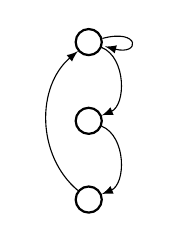
\begin{tikzpicture}[>=latex]
            \node[draw, thick, circle, radius=0.4] (a) at (0,0) {$\cX\cH\cH$};
            \node[draw, thick, circle, radius=0.4] (b) at (0,-1) {$\cH\cH\cM$};
            \node[draw, thick, circle, radius=0.4] (c) at (0,-2) {$\cH\cM\cH$};
            \draw[->] (a) edge [loop right] node[right] {$\cH$} (a);
            \draw[->] (a) edge [bend left=67.5] node[right] {$\cM$} (b);
            \draw[->] (b) edge [bend left=67.5] node[right] {$\cH$} (c);
            \draw[->] (c) edge [bend left=50] node[left] {$\cH$} (a);
        \end{tikzpicture}

        (Example~\ref{ex:auto-kill})\\[1pt]
        $\lambda^{\strat} = \overbar{\binom{1}{3}}^{\text{Kill}}$
    \end{center}
\end{minipage}
%
    \begin{minipage}[c]{0.48\textwidth}
    \begin{center}
        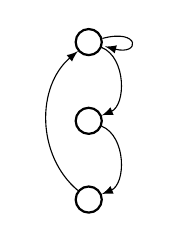
\begin{tikzpicture}[>=latex]
            \node[draw, thick, circle, radius=0.4] (a) at (0,0) {$\cX\cT\cH$};
            \node[draw, thick, circle, radius=0.4] (b) at (0,-1) {$\cT\cH\cM$};
            \node[draw, thick, circle, radius=0.4] (c) at (0,-2) {$\cH\cM\cR$};
            \draw[->] (a) edge [loop right] node[right] {$\cH$} (a);
            \draw[->] (a) edge [bend left=67.5] node[right] {$\cM$} (b);
            \draw[->] (b) edge [bend left=67.5] node[right] {$\cR$} (c);
            \draw[->] (c) edge [bend left=50] node[left] {$\cH$} (a);
        \end{tikzpicture}

        (Example~\ref{ex:auto-skip})\\[1pt]
        $\lambda^{\strat} = \overbar{\binom{1}{3}}^{\text{Skip-Next}}$
    \end{center}
\end{minipage}
%
    \caption{Automata $\GG{\lambda^{\strat}}$ for Examples 1 and 2.}
    \label{fig:min-graph}
\end{figure}

\afterpage{%
    \clearpage
   \begin{figure*}[h]
       \begin{minipage}[c]{0.4\textwidth}
    \begin{center}
        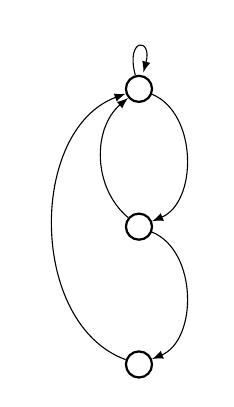
\begin{tikzpicture}[>=latex]
            \node[draw, thick, circle, radius=0.4] (a) at (0,0) {$\textcolor{white}{\cH}\cX\cX\cH\textcolor{white}{\cH}$};
            \node[draw, thick, circle, radius=0.4] (b) at (0,-1.75) {$\textcolor{white}{\cH}\cX\cH\cM\textcolor{white}{\cH}$};
            \node[draw, thick, circle, radius=0.4] (c) at (0,-3.5) {$\textcolor{white}{\cH}\cH\cM\cM\textcolor{white}{\cH}$};
            \draw[->] (a) edge [loop above] node[above] {$\cH$} (a);
            \draw[->] (a) edge [bend left=67.5] node[right] {$\cM$} (b);
            \draw[->] (b) edge [bend left=50] node[left] {$\cH$} (a);
            \draw[->] (b) edge [bend left=67.5] node[right] {$\cM$} (c);
            \draw[->] (c) edge [bend left=70] node[left] {$\cH$} (a);
        \end{tikzpicture}

        (Constraint 1)\\[1pt]
        $\lambda^{\strat}_1 = \overbar{\left<2\right>}^{\text{Kill}}$
    \end{center}
\end{minipage}
\hspace{1cm}
\begin{minipage}[c]{\textwidth}
    \begin{center}
        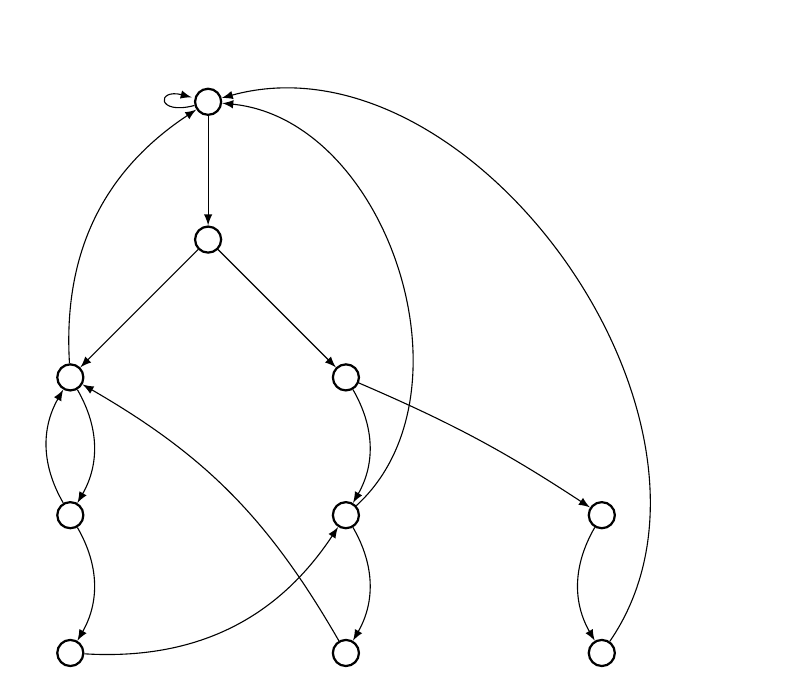
\begin{tikzpicture}[>=latex]
            \node[draw, thick, circle, radius=0.4] (a) at (0,0) {$\cX\cX\cX\cH\cH$};
            \node[draw, thick, circle, radius=0.4] (b) at (0,-1.75) {$\cX\cX\cH\cH\cM$};
            \node[draw, thick, circle, radius=0.4] (c) at (-1.75,-3.5) {$\cX\cX\cH\cM\cH$};
            \node[draw, thick, circle, radius=0.4] (d) at (-1.75,-5.25) {$\cX\cH\cM\cH\cM$};
            \node[draw, thick, circle, radius=0.4] (e) at (-1.75,-7) {$\cH\cM\cH\cM\cM$};
            \node[draw, thick, circle, radius=0.4] (f) at (1.75,-3.5) {$\cX\cH\cH\cM\cM$};
            \node[draw, thick, circle, radius=0.4] (g) at (1.75,-5.25) {$\cX\cH\cM\cM\cH$};
            \node[draw, thick, circle, radius=0.4] (h) at (1.75,-7) {$\cH\cM\cM\cH\cM$};
            \node[draw, thick, circle, radius=0.4] (i) at (5,-5.25) {$\cH\cH\cM\cM\cM$};
            \node[draw, thick, circle, radius=0.4] (j) at (5,-7) {$\cH\cM\cM\cM\cH$};

            \draw[->] (a) edge [loop left] node[left] {$\cH$} (a);
            \draw[->] (a) edge [] node[right] {$\cM$} (b);
            \draw[->] (b) edge node [above] {$\cH$} (c);
            \draw[->] (b) edge node [above] {$\cM$} (f);
            \draw[->] (c) edge [bend left] node [left] {$\cH$} (a);
            \draw[->] (c) edge [bend left] node [right] {$\cM$} (d);
            \draw[->] (d) edge [bend left] node [left] {$\cH$} (c);
            \draw[->] (d) edge [bend left] node [right] {$\cM$} (e);
            \draw[->] (e) edge [bend right] node [below] {$\cH$} (g);
            \draw[->] (f) edge [bend left] node [right] {$\cH$} (g);
            \draw[->] (f) edge [bend left=5] node [above] {$\cM$} (i);
            \draw[->] (g) edge [bend right = 66] node [right] {$\cH$} (a);
            \draw[->] (g) edge [bend left] node [right] {$\cM$} (h);
            \draw[->] (h) edge [bend right = 15] node [above] {$\cH$} (c);
            \draw[->] (i) edge [bend right] node [left] {$\cH$} (j);
            \draw[->] (j) edge [bend right = 70] node [right] {$\cH$} (a);

        \end{tikzpicture}

        (Constraint 2)\\[1pt]
        $\lambda^{\strat}_2 = \overbar{\binom{3}{5}}^{\text{Kill}}$
    \end{center}
\end{minipage}
\hspace{1cm}
\begin{minipage}[c]{0.8\textwidth}
    \begin{center}
        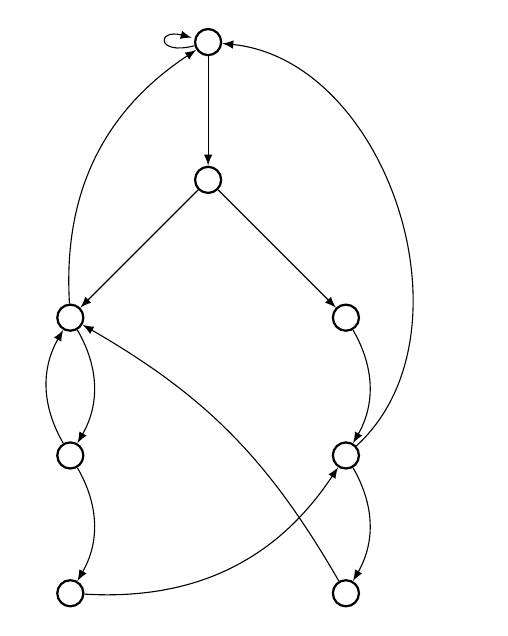
\begin{tikzpicture}[>=latex]
            \node[draw, thick, circle, radius=0.4] (a) at (0,0) {$\cX\cX\cX\cH\cH$};
            \node[draw, thick, circle, radius=0.4] (b) at (0,-1.75) {$\cX\cX\cH\cH\cM$};
            \node[draw, thick, circle, radius=0.4] (c) at (-1.75,-3.5) {$\cX\cX\cH\cM\cH$};
            \node[draw, thick, circle, radius=0.4] (d) at (-1.75,-5.25) {$\cX\cH\cM\cH\cM$};
            \node[draw, thick, circle, radius=0.4] (e) at (-1.75,-7) {$\cH\cM\cH\cM\cM$};
            \node[draw, thick, circle, radius=0.4] (f) at (1.75,-3.5) {$\cX\cH\cH\cM\cM$};
            \node[draw, thick, circle, radius=0.4] (g) at (1.75,-5.25) {$\cX\cH\cM\cM\cH$};
            \node[draw, thick, circle, radius=0.4] (h) at (1.75,-7) {$\cH\cM\cM\cH\cM$};

            \draw[->] (a) edge [loop left] node[left] {$\cH$} (a);
            \draw[->] (a) edge [] node[right] {$\cM$} (b);
            \draw[->] (b) edge node [above] {$\cH$} (c);
            \draw[->] (b) edge node [above] {$\cM$} (f);
            \draw[->] (c) edge [bend left] node [left] {$\cH$} (a);
            \draw[->] (c) edge [bend left] node [right] {$\cM$} (d);
            \draw[->] (d) edge [bend left] node [left] {$\cH$} (c);
            \draw[->] (d) edge [bend left] node [right] {$\cM$} (e);
            \draw[->] (e) edge [bend right] node [below] {$\cH$} (g);
            \draw[->] (f) edge [bend left] node [right] {$\cH$} (g);
            \draw[->] (g) edge [bend right = 66] node [right] {$\cH$} (a);
            \draw[->] (g) edge [bend left] node [right] {$\cM$} (h);
            \draw[->] (h) edge [bend right = 15] node [above] {$\cH$} (c);

        \end{tikzpicture}

        (Result)\\[1pt]
        $\Lambda^{\strat}_0 = \left\{ \lambda^{\strat}_1,\, \lambda^{\strat}_2 \right\}$
    \end{center}
\end{minipage}

       \caption{Automata $\GG{\lambda^{\strat}_1}^*$, $\GG{\lambda^{\strat}_2}^*$, and $\GG{\Lambda^{\strat}_0}^*$ for Example~\ref{ex:auto-comb}.}
       \label{fig:multi-graphs}
   \end{figure*}
    \clearpage
}

\begin{example}%
    \label{ex:auto-kill}%
    Given an \ewhc{}, $\lambda^{\strat} = \overbar{\binom{1}{3}}^{\text{Kill}}$, the automaton $\GG{\lambda^{\strat}}^*$ is shown in the left-hand side of Figure~\ref{fig:min-graph}.
    The vertex represented by the word $\cX\cH\cH$ is obtained by merging $\cH\cH\cH$ and $\cM\cH\cH$.
\end{example}

\begin{example}%
    \label{ex:auto-skip}%
    Given an \ewhc{}, $\lambda^{\strat} = \overbar{\binom{1}{3}}^{\text{Skip-Next}}$, the automaton $\GG{\lambda^{\strat}}^*$ is shown in the right-hand side of Figure~\ref{fig:min-graph}.
\end{example}

The minimal automaton for Kill and Skip-Next in Figure~\ref{fig:min-graph} have identical number of vertices but slightly different transitions.
This is not a coincidence, but follows directly from Definition~\ref{def:new-mk} and the extended alphabet $\Sigma\left(\strat\right)$.
Since we build the automaton using the job completion character $\cT$, both automata will always have the same structure.
It is only the first job completion, after a period of no job completions ($\cM$), that differ.
We emphasise that despite the extended automaton model appear similar for the Kill and Skip-Next strategies, the differing transitions of the two automata significantly affect the corresponding closed-loop systems, as will be clear in Section~\ref{sec:stability}.


The \tool{} automaton model can also handle the case where a task $\tau$ is subject to a set of multiple constraints.
Intuitively, building upon Definition~\ref{def:satisfaction}, the satisfaction set of $\Lambda^{\strat}$ can be derived as follows:
%
\begin{equation}
    \label{eq:satisfaction-multi}
    \sset{N}{\Lambda^{\strat}} = \bigcap_{\lambda^{\strat}_i \in \Lambda^{\strat}_0} \sset{N}{\lambda^{\strat}_i}, \quad N \geq 1.
\end{equation}
%
With the notion of a satisfaction sets for sets of \ewhc{}, it is trivial to see that the domination relations also hold (Definition~\ref{def:domination}).
Since the stability analysis presented in this paper is invariant to the type (and amount) of constraints acting on the control task $\tau$, we henceforth say that $\tau$ is subject to a set of \ewhc{} $\Lambda^\strat$ (unless stated otherwise).
%
\begin{example}%
    \label{ex:auto-comb}%
    Given two \ewhc{}, $\lambda^{\strat}_1 = \overbar{\left<2\right>}^{\text{Kill}}$ and $\lambda^{\strat}_2 = \overbar{\binom{3}{5}}^{\text{Kill}}$, the automata $\GG{\lambda^{\strat}_1}^*$ and $\GG{\lambda^{\strat}_2}^*$ are shown as the leftmost and middle automata of Figure~\ref{fig:multi-graphs}.
    Generating the automaton $\GG{\Lambda^{\strat}_0}^*$ from the set $\Lambda^{\strat} = \{ \lambda^{\strat}_1, \lambda^{\strat}_2 \}$ results in the rightmost automaton of Figure~\ref{fig:multi-graphs}, satisfying both $\lambda^{\strat}_1$ and $\lambda^{\strat}_2$.
    \fix{}
\end{example}


\subsection{Dynamic model of a graph}
\label{ssec:dynamicgraph}

Extracting all the transitions in $\EE{\Lambda^\strat}$ corresponding to a character $\event$ yields what is generally known as a \emph{directed adjacency matrix}~\cite{xu2012matrix}, denoted here as a \emph{transition matrix}.
\begin{definition}[Transition matrix]%
    \label{def:transition}%
    Given an automaton $\GG{\Lambda^\strat}$, the \emph{transition matrix} $F_{\event} ( \GG{\Lambda^\strat} ) \in \R^{\abs{\VV{\Lambda^\strat}} \times \abs{\VV{\Lambda^\strat}}}$ with $\event\in\Sigma\left(\strat\right)$, is computed as $F_{\event} ( \GG{\Lambda^\strat} ) = \{f_{i,j}(\event)\}$ with
    %
    \begin{equation*}
        f_{i,j}\funof{\event}=
        \begin{cases}
            1, &\text{ if } \exists \, e=(v_j,v_i,\event) \in \EE{\Lambda^\strat} \\
            0, &\text{ otherwise.}
        \end{cases}
        \end{equation*}%
\end{definition}
%
Since there can only exist \emph{at most one} successor from each vertex with a transition labeled with $\event$, the transition matrix $F_\event$ will thus have a column sum of either 1 or 0.
We introduce a vector $q_t\in \R^{\abs{\VV{\Lambda^\strat}}}$ called the \emph{G-state} (for graph state), representing the state of the given automaton $\GG{\Lambda^\strat}$, which is associated to the interval $\pi_t$.
This vector is formally defined as follows.
\begin{definition}[G-state $q_t$]%
    \label{def:qt}%
    Given an automaton $\GG{\Lambda^\strat} = (\VV{\Lambda^\strat}, \EE{\Lambda^\strat})$ and a word $\aword \in \Sigma\left( \strat \right)^N$, for $k = \abs{v},\,\, v\in\VV{\Lambda^\strat}$, we define $q_t\in \R^{\abs{\VV{\Lambda}}}$, where the $i$-th element $q_{t,i}$ is defined as:
    \begin{equation*}
        q_{t,i}=
        \begin{cases}
            1, &\text{ if } \aword\left(t-k..t-1\right) \equiv v_i \in \VV{\Lambda^\strat} \\
            0, &\text{otherwise}.
        \end{cases}
    \end{equation*}
\end{definition}
In other words, the G-state $q_t$ is the vector representation of the vertex we are \emph{leaving} at step $t$.
In this definition, $q_t=0$ means that the transition at step $t-1$ was infeasible for the automaton.
The G-state dynamics, given an arbitrary word $\aword=\{\alpha_1,\dots,\alpha_t,\dots,\}$, is then defined as $q_{t+1} = F_{\event} ( \GG{\Lambda^\strat} )\cdot q_t$.
Hence, the following property from~\cite{xu2012matrix} holds.
\begin{lemma}[Infeasible sequence]
    \label{cor:Fseqnotinlambda}
    If $\aword \notin \sset{N}{ \Lambda^\strat }$, then $F_{\aword} ( \GG{\Lambda^\strat} ) =
    F_{\event_N} ( \GG{\Lambda^\strat} )\cdots F_{\event_2} ( \GG{\Lambda^\strat} )\cdot F_{\event_1} ( \GG{\Lambda^\strat} ) = 0$
\end{lemma}
Thus, if $q_t=0$ for any $t$, then $q_{t'}=0$ for $t' \geq t$.


\section{Stability Analysis}
\label{sec:stability}
Using the alphabet $\Sigma\left(\strat\right)$ and the chosen actuator mode (i.e., zeroing, or holding the previous value), we compute the closed-loop behaviour of the controlled system.
We identify one matrix for each dynamics corresponding to an interval $\pi_t$ associated by $\alpha \in \Sigma\left( \strat \right)$, building the set $\Aa^\strat$.

\textbf{\tK{}: }%
%
We define $\tilde x_t^{\,\text{K}} = \left[ x_t^\T{}\,\, z_t^\T{}\,\, u_t^\T{} \right]^\T{}$ as the closed-loop state vector and compute the closed-loop dynamics $\clmat{}^{\,\text{K}}_{\cH}$, corresponding to the character $\cH$.
\begin{equation*}
    \tilde x_{t+1}^{\,\text{K}} = \clmat{}^{\,\text{K}}_{\cH}\,\tilde x_t^{\,\text{K}}, \quad
    \clmat{}^{\,\text{K}}_{\cH} = \begin{bmatrix}
        \Ap       & 0    & \Bp       \\
        -\Bc\Cp   & \Ac  & -\Bc\Dp   \\
        -\Dc\Cp   & \Cc  & -\Dc\Dp   \\
    \end{bmatrix}
\end{equation*}
%
For the case of $\cM$, the controller execution terminates prematurely, thus not updating its states ($z_{t+1} = z_t$).
Depending on the actuation mode, the controller output is either zeroed ($u_{t+1} = 0$) or held ($u_{t+1} = u_t$).
The resulting closed-loop system in state-space form is denoted with $\clmat{}^{\,\text{K}}_{\cM}$:
\begin{equation*}
    \tilde x_{t+1}^{\,\text{K}} = \clmat{}^{\,\text{K}}_{\cM}\,\tilde x_t^{\,\text{K}}, \quad
    \clmat{}^{\,\text{K}}_{\cM} = \begin{bmatrix}
        \Ap & 0  & \Bp \\
        0   & I  & 0   \\
        0   & 0  & \Delta
    \end{bmatrix}
\end{equation*}
Here, $\Delta = I$ (identity matrix) if the control signal is held and $\Delta = 0$ if it is zeroed.
The set of dynamic matrices that a controlled system under the \tK{} strategy may experience is then $\Aa^{\text{\tK{}}}=\left\{\clmat{}^{\,\text{K}}_{\cH},\clmat{}^{\,\text{K}}_{\cM}\right\}$.

\textbf{\tS{}: }%
%
For the \tS{} strategy, we introduce two additional states $\hat x_t$ and $\hat u_t$ storing the old values of $x_t$ and $u_t$ while the controller awaits an update.
The resulting state vector then becomes $\tilde x_t^{\,\text{S}} = \left[ x_t^\T{}\,\,z_t^\T{}\,\, u_t^\T{}\,\, \hat{x}_t^\T{}\,\, \hat{u}_t^\T{} \right]^\T{}$.
When $\pi_t$ is associated to $\cH$, the two additional states mirror the behaviour of the states of which they are storing data.
The resulting closed-loop system is described using $\clmat{}^{\,\text{S}}_{\cH}$:
%
\begin{equation*}
    \tilde x_{t+1}^{\,\text{S}} = \clmat{}^{\,\text{S}}_{\cH}\,\tilde x_t^{\,\text{S}}, \quad
    \clmat{}^{\,\text{S}}_{\cH} = \begin{bmatrix}
        \Ap       & 0    & \Bp      & 0 & 0 \\
        -\Bc\Cp   & \Ac  & -\Bc\Dp  & 0 & 0 \\
        -\Dc\Cp   & \Cc  & -\Dc\Dp  & 0 & 0 \\
        \Ap       & 0    & \Bp      & 0 & 0 \\
        -\Dc\Cp   & \Cc  & -\Dc\Dp  & 0 & 0 \\
    \end{bmatrix}.
\end{equation*}
%
For the case of $\cM$ in $\pi_t$ the two augmented states hold their previous values.
The resulting closed-loop system is described by $\clmat{}^{\,\text{S}}_{\cM}$:
%
\begin{equation*}
    \tilde x_{t+1}^{\,\text{S}} = \clmat{}^{\,\text{S}}_{\cM}\,\tilde x_t^{\,\text{S}}, \quad
    \clmat{}^{\,\text{S}}_{\cM}=\begin{bmatrix}
        \Ap & 0  & \Bp & 0 & 0 \\
        0   & I  & 0   & 0 & 0 \\
        0   & 0  & \Delta   & 0 & 0 \\
        0   & 0  & 0   & I & 0 \\
        0   & 0  & 0   & 0 & I \\
    \end{bmatrix}.
\end{equation*}
%
Finally, for the case of recovery $\cR$ in $\pi_t$, the new control command is calculated using the values stored in $\hat x_t$ and $\hat u_t$.
The resulting closed-loop system is described by $\clmat{}^{\,\text{S}}_{\cR}$:
%
\begin{equation*}
    \tilde x_{t+1}^{\,\text{S}} = \clmat{}^{\,\text{S}}_{\cR} \, \tilde x_{t}^{\,\text{S}}, \quad
    \clmat{}^{\,\text{S}}_{\cR} = \begin{bmatrix}
        \Ap & 0    & \Bp & 0       & 0 \\
        0   & \Ac  & 0   & -\Bc\Cp & -\Bc\Dp \\
        0   & \Cc  & 0   & -\Dc\Cp & -\Dc\Dp \\
        \Ap & 0    & \Bp & 0       & 0 \\
        0   & \Cc  & 0   & -\Dc\Cp & -\Dc\Dp \\
    \end{bmatrix}.
\end{equation*}
%
The set of dynamic matrices under the \tS{} strategy is then defined as $\Aa^{\text{\tS{}}}=\left\{\clmat{}^{\,\text{S}}_{\cH},\clmat{}^{\,\text{S}}_{\cM},\clmat{}^{\,\text{S}}_{\cR}\right\}$.

\subsection{Kronecker Lifted Switching System}%
\label{sec:system_dynamics}
%
A straightforward approach to analyse the switching system's ($\Aa^\strat$) stability under any switching pattern constrained by $\Lambda^\strat$ would be configuring a CJSR problem in the form of Equation~\eqref{cjsr}, obtaining $\rho\,(\Aa^\strat,\GG{\Lambda^\strat})$.
However, few efficient CJSR computation methods exist.

Instead, building upon the recent work of~\cite{xu2020approximation}, we seek to obtain an equivalent system model based on \emph{Kronecker lifting}~\cite{horn2012matrix}, characterized by a set of matrices denoted by $\Alifted_{\Lambda^\strat}$ and behaving as an \emph{arbitrary switching system}, such that $\rho\funof{\Alifted_{\Lambda^\strat}} = \rho\funof{\Aa^{\strat},\GG{\Lambda^\strat}}$.
This way, powerful algorithms applicable to arbitrary switching system~\cite{vankeerberghen2014jsr,sparsejsr} can be used to find tight stability bounds.
%
By leveraging the vector $q_t$ of Definition~\ref{def:qt}, we introduce the \emph{lifted discrete-time state}, $\xi_t\in\R^{n\cdot n_{\VV{}}}$, defined as 
\begin{equation*}
    \xi_t = q_t\otimes \tilde x_t,
\end{equation*}
where $n$ is the number of closed-loop states $\tilde x_t$, $n_{\VV{}} = \abs{\VV{\Lambda^\strat}}$, and $\otimes$ is the Kronecker product operator.
By construction, $\xi_t$ is then a vector composed of $n_{\VV{}}$ blocks of size $n$, where at most one block is equal to $\tilde x_t$ and all other blocks are equal to the $0$ vector.
%
\fix{P is problematic here}
Then, we build a set of lifted matrices $P_{\alpha} ( \GG{\Lambda^\strat} )\in\R^{n\cdot n_{\VV{}}\times n\cdot n_{\VV{}}}$ that includes information about both the system dynamics and the possible transitions given a certain outcome $\alpha \in \Sigma\left(\strat\right)$:
%
\begin{equation*}
    P_{\alpha} ( \GG{\Lambda^\strat} ) = F_{\alpha} ( \GG{\Lambda^\strat} )\otimes \clmat{}_\alpha^\strat,\quad \alpha \in \Sigma \left( \strat \right).
\end{equation*}
%
The lifted dynamics of the closed loop system then become%
%
\begin{equation*}
    \xi_{t+1} = P_{\alpha} ( \GG{\Lambda^\strat} )\,\xi_t.
\end{equation*}
%
Formally, we obtain an equivalent closed-loop system composed of a set of lifted dynamic matrices, $\Alifted_{\Lambda^\strat}$.
%
\begin{definition}[Lifted switching set $\Alifted_{\Lambda^\strat}$]%
    \label{def:switching_set}%
    Given a set of dynamic matrices $\Aa^{\strat}$ and an automaton $\GG{\Lambda^\strat}$, the switching set $\Alifted_{\Lambda^\strat}$ is defined as the set of all lifted matrices corresponding to $\Aa^{\strat}$.
    Formally,
    %
    \begin{equation*}
        \Alifted_{\Lambda^\strat} = \left\{ P_{\alpha} ( \GG{\Lambda^\strat} ) \,\, | \,\, \alpha \in \Sigma\left(\strat\right) \right\}.
    \end{equation*}
\end{definition}
%
By leveraging the mixed-product property~\cite{horn2012matrix} of $\otimes$ and by introducing a proper submultiplicative norm, it is possible to prove that $\rho\left(\Alifted_{\Lambda^\strat}\right)= \rho\,(\Aa^{\strat},\GG{\Lambda^\strat})$.
For more details and a formal proof we refer the interested reader to~\cite{xu2020approximation}.


\subsection{Extended Weakly Hard and JSR Properties}
\label{sec:analytic_results}
%
We now provide a general relation between \emph{all} \ewhc{}s in terms of the joint spectral radii.

\begin{theorem}[JSR dominance]%
    \label{th:rho_dominance_general}%
    Given two arbitrary \ewhc{}, $\lambda_1^\strat$ and $\lambda_2^\strat$.
    If $\lambda_1^\strat \preceq \lambda_2^\strat$, then
    \begin{equation*}
        \rho\funof{\Alifted_{\lambda_1^\strat}} \leq \rho\funof{\Alifted_{\lambda_2^\strat}}.
    \end{equation*}

    \begin{proof}
        \fix{Add an explanation that the second part of the equation below holds because of the mixed-product property of $\otimes$, because otherwise $\clmat{}$ might be confusing}
        From Equation~\eqref{jsr}, for a generic \ewhc{} $\lambda^\strat$,
        \begin{equation*}
            \rho\left(\Alifted_{\lambda^\strat}\right) = \lim_{\ell\rightarrow \infty}\rho_\ell\left(\Alifted_{\lambda^\strat}\right), \quad \rho_\ell\left(\Alifted_{\lambda^\strat}\right) = \max_{w \in \sset{\ell}{\lambda^\strat}}\norm{\clmat{}_{w}}^{1/\ell}.
        \end{equation*}
        According to Definition~\ref{def:domination}, it holds that $\lambda^\strat_1 \preceq \lambda^\strat_2$ if and only if $\sset{}{\lambda^\strat_1} \subseteq \sset{}{\lambda^\strat_2}$.
        Thus, if for a word $a$ it holds that $a \in \sset{\ell}{\lambda^\strat_1}$, then it also holds that $a \in \sset{\ell}{\lambda^\strat_2}$.
        The set of all possible $\clmat{}_{a}$ is thus included in the set of all possible $\clmat{}_{b},\, b \in \sset{\ell}{\lambda^\strat_2}$.
        As a consequence it holds that
        \begin{equation*}
            \max_{a \in \sset{\ell}{\lambda^\strat_1}}\norm{\clmat{}_{a}}^{1/\ell} \leq
            \max_{b \in \sset{\ell}{\lambda^\strat_2}}\norm{\clmat{}_{b}}^{1/\ell}, \quad
            \forall \ell\in\mathbb{N}^{>}.
        \end{equation*}
        The theorem follows immediately when $\ell\rightarrow \infty$.
    \end{proof}
\end{theorem}

Theorem~\ref{th:rho_dominance_general} is the first result that provides a clear, analytic, correlation between the control theoretical analysis and real-time implementation.
Primarily, it implies that the constraint dominance from Definition~\ref{def:domination} also carries on to the JSR, giving us a notion of \emph{JSR dominance}.
If stability under a specific \ewhc{} is shown, Theorem~\ref{th:rho_dominance_general} guarantees stability for all \ewhc{} which are harder to satisfy.
The results of Theorem~\ref{th:rho_dominance_general} are strategy independent, further reducing the coupling between the control analysis and implementation approach.
Additionally, the results are independent of the dynamics and apply to open-loop as well as closed-loop systems, including feedforward controllers and any linear feedback control strategy -- provided that an appropriate reformulation of matrices $\Aa^\strat$ is given.

Two Corollaries of Theorem~\ref{th:rho_dominance_general} are derived for the commonly used models $\erowmiss{}{\strat}$ and $\eanymiss{}{\strat}$, highlighting some practical relations between such constraints.
\begin{corollary}[$\eanymiss{}{\strat}$ dominance]%
    \label{cor:rho_dominance_mk}%
    Given two \ewhc{}, $\lambda^\strat_1 = \overbar{\binom{x}{k_1}}^{\strat}$ and $\lambda^\strat_2 = \overbar{\binom{x}{k_2}}^{\strat}$, if $k_1 \leq k_2$ then
    \begin{equation*}
        \rho\bigl(\Alifted_{\lambda^\strat_2}\bigr) \leq \rho\bigl(\Alifted_{\lambda^\strat_1}\bigr).
    \end{equation*}
    %
    \begin{proof}
        According to~\cite{Wu:2020}, $\overbar{\binom{x}{k_2}}^{\strat}\preceq\overbar{\binom{x}{k_1}}^{\strat}$ if $k_1 \leq k_2$.
        The corollary follows directly from~\cite{Wu:2020} and Theorem~\ref{th:rho_dominance_general}.
    \end{proof}
\end{corollary}
%
\begin{corollary}[$\erowmiss{}{\strat}$ dominance]%
    \label{cor:rho_dominance_cons}%
    Given two \ewhc{}, $\lambda^\strat_1 = \erowmiss{}{\strat}$ and $\lambda^\strat_2 =\eanymiss{}{\strat}$, then
    \begin{equation*}
        \rho\bigl(\Alifted_{\lambda^\strat_2}\bigr) \leq \rho\bigl(\Alifted_{\lambda^\strat_1}\bigr).
    \end{equation*}
    %
    \begin{proof}
        According to~\cite{Maggio:2020} it holds that $\erowmiss{}{\strat} \equiv \overbar{\binom{x}{x+1}}^{\strat}$.
        The corollary follows directly from~\cite{Maggio:2020} and Corollary~\ref{cor:rho_dominance_mk}.
    \end{proof}
\end{corollary}
%
The conclusions drawn from Theorem~\ref{th:rho_dominance_general} are theoretical, but its practical applicability lies in the algorithm used to find $\rho^{LB}$ and $\rho^{UB}$, i.e., lower and upper bounds for the JSR value.
Using these bounds we can determine the stability of the corresponding switching systems, as follows:
%
$$
\rho^{LB} \bigl( \Alifted_{\lambda^\strat_1} \bigr) \leq \rho \bigl( \Alifted_{\lambda^\strat_1} \bigr) \leq \rho \bigl( \Alifted_{\lambda^\strat_2} \bigr) \leq \rho^{UB} \bigl( \Alifted_{\lambda^\strat_2} \bigr).
$$
%
Regardless of the algorithm used to find the bounds, we can generally conclude that if $\rho^{UB} \left( \Alifted_{\lambda^\strat} \right) < 1$ the constrained system is switching stable.
Similarly, if $\rho^{LB} \left( \Alifted_{\lambda^\strat} \right) > 1$ the system is unstable.
Thus, if $\lambda^\strat_1 \preceq \lambda^\strat_2$, where $\rho^{UB} \left( \Alifted_{\lambda^\strat_2} \right) < 1$, we know that the system under $\lambda^\strat_1$ constraints is switching stable.
A similar relation holds for the lower bound.

We now extend the results of Theorem~\ref{th:rho_dominance_general} by relating the joint spectral radius of a single constraint to sets of constraints.
\begin{theorem}%
    \label{th:rho_dominance_set_general}%
    Given an arbitrary \ewhc{} $\lambda^\strat$, it holds that
    \begin{equation*}
        \rho\left(\Alifted_{\Lambda^\strat}\right) \leq \rho \left( \Alifted_{\lambda^\strat} \right) ,\,\, \forall \Lambda^\strat \ni \lambda^\strat.
    \end{equation*}
    %
    \begin{proof}
        \fix{Add an explanation that the second part of the equation below holds because of the mixed-product property of $\otimes$, because otherwise $\clmat{}$ might be confusing}
        For an arbitrary \ewhc{} set $\Lambda^\strat = \{\lambda^\strat_1, \dots, \lambda^\strat_N\}$, its satisfaction set is $\sset{\ell}{\Lambda^\strat} = \bigcap_{i \in \{1,\dots, N\}} \sset{\ell}{\lambda^\strat_i}$.
        Thus, for any $\lambda^\strat \in \Lambda^\strat$ it holds that 
        \begin{equation*}
            \sset{\ell}{\Lambda^\strat} \subseteq \sset{\ell}{\lambda^\strat}
        \end{equation*}
        If a word $a$ is in $\sset{\ell}{\Lambda^\strat}$ it also belongs to $\sset{\ell}{\lambda^\strat}$. 
        The set of all possible $\clmat{}_{a}$ is thus included in the set of all possible $\clmat{}_{b},\, b \in \sset{\ell}{\lambda^\strat}$.
        As a consequence it holds that
        \begin{equation*}
            \max_{a \in \sset{\ell}{\Lambda^\strat }} \norm{\clmat{}_{a}}^{1/\ell} \leq
            \max_{b \in \sset{\ell}{\lambda^\strat }} \norm{\clmat{}_{b}}^{1/\ell}, \quad
            \forall \ell\in\mathbb{N}^{>}.
        \end{equation*}
        The theorem follows immediately when $\ell\rightarrow \infty$.
    \end{proof}
\end{theorem}

As in Theorem~\ref{th:rho_dominance_general}, the more we restrict the execution pattern of the control task with sets of constraints, the lower its JSR will be.
Theorem~\ref{th:rho_dominance_set_general} delivers the practical insight that enforcing tighter \ewhc{} to a stable system will \emph{never} destabilise it, as formally stated in the following corollary.
\begin{corollary}%
    \label{cor:rho_dominance_set}%
    Given an arbitrary \ewhc{}, $\lambda^\strat$, if $\rho \left( \Alifted_{\lambda^\strat} \right) < 1$ then
    \begin{equation*}
        \rho\left(\Alifted_{\Lambda^\strat}\right) < 1 ,\,\, \forall \Lambda^\strat \ni \lambda^\strat.
    \end{equation*}

    \begin{proof}
        The corollary follows immediately from Theorem~\ref{th:rho_dominance_set_general} when $\rho \left( \Alifted_{\lambda^\strat} \right) < 1$.
    \end{proof}
\end{corollary}


\section{Evaluation}
\label{sec:evaluation}
We now apply the lifted dynamics model presented in Section~\ref{sec:stability} to two representative case studies.
The corresponding controllers are designed to stabilise the closed loop in ideal conditions, i.e., without deadline misses.
Numerical experiments are performed to analyse the stability of the control systems subject to different constraints, particularly the $\eanymiss{}{\strat}$ constraints.
We consider all combinations of strategy (\tK{} or \tS{}) and actuator mode (\tZ{} or \tH{}).

For each combination of control system and \ewhc{}, $\lambda^{\strat}$, the lifted set $\Alifted_{\lambda^\strat}$ is generated.
We approximate the JSR of $\Alifted_{\lambda^\strat}$ using three different algorithms.
First, a lower and upper bound of $\rho \left( \Alifted_{\lambda^\strat} \right)$ are computed using the \code{JSR toolbox}~\cite{vankeerberghen2014jsr}.
We compare these bounds with an upper bound of the JSR obtained via SOS relaxations, described in Section~\ref{sec:existing}; both the \emph{dense} and \emph{sparse} algorithm from the \code{SparseJSR} toolbox~\cite{sparsejsr} are executed, obtaining $\rho_{\sos,2d}\left(\Alifted_{\lambda^\strat}\right)$ and $\rho_{\textrm{TSSOS},2d}\left(\Alifted_{\lambda^\strat}\right)$ respectively.
%
For efficiency, we run experiments at the first relaxation order $d = 1$.

The \code{JSR toolbox} provides an accurate lower bound and a coarse upper bound in a few seconds.
In contrast, the dense SOS-based method usually finds a good upper bound but takes more time.
The sparse/dense upper bounds are obtained with the \code{SparseJSR} Julia package.
Since \code{JSR toolbox} and \code{SparseJSR} are implemented in different programming languages (Matlab and Julia) and rely on different SDP solvers (SDPT3/SeDuMi and MOSEK), it is not meaningful to compare their respective timings.
However, the time it takes to run the dense and sparse SOS methods in Julia is compared.
All numerical examples have been computed on an Intel Core i5-8265U@1.60GHz CPU with 8GB RAM memory.

\subsection{Process Industrial Plant}\label{sec:eval:stable}
We here analyse a stable discrete-time plant $\plant_1$, representative of the process industry~\cite{Hagglund:2002}, controlled using a PI-controller $\ctrler_1$ (sampled using the sampling period $\Ts = 0.5$~s):
\begin{equation*}
    %plant = batch 4, ID 1
    \begin{aligned}
        \plant_1: \,\, &\left\{
        \begin{aligned}
            x_{t+1} &= \begin{bmatrix}
                0.606 & 0.304 & 0.076 \\
                0 & 0.606 & 0.304 \\
                0 & 0 & 0.606 \\
            \end{bmatrix} x_t + \begin{bmatrix}
                0.014 \\
                0.091 \\
                0.394 \\
            \end{bmatrix} u_t \\
            y_t &= \begin{bmatrix}
                1 & 0 & 0
            \end{bmatrix} x_t
        \end{aligned} \right. \\
        \ctrler_1: \,\, &\left\{
        \begin{aligned}
            z_{t+1} &= z_t + 0.359\, y_t \\
            u_{t+1} &= 0.454\, z_t + 0.633\, y_t
        \end{aligned} \right.
    \end{aligned}
\end{equation*}

\afterpage{
    \clearpage
    \begin{landscape}
        % TABLE FOR STABLE SYSTEM
        \begin{table}
\vspace{1.5cm}
\setlength{\tabcolsep}{5pt}
\renewcommand{\arraystretch}{1.25}
\caption{Results obtained for the stable system $\plant$, when controlled using $\ctrler$.}\label{table:stable}
\rowcolors{2}{light-table-colour}{white}
\begin{center}
\resizebox{1.5\textwidth}{!}{%
\begin{tabular}{|cc|lllll|lllll|lllll|lllll|}
\hline
% \rowcolor{gray!50}
% &&\multicolumn{3}{c}{Dense $d=1$}&\multicolumn{3}{c}{Sparse $d=1$} &\multicolumn{2}{c}{JSR\_toolbox}\\
% \rowcolor{gray!50}
% \multirow{-2}*{$m$}&\multirow{-2}*{$k$}&$ub$&time&$mb$&$ub$&time&$mb$&$lb$&$ub$\\
\rowcolor{dark-table-colour}
& & \multicolumn{5}{c|}{\textbf{\tKZ{}}} & \multicolumn{5}{c|}{\textbf{\tKH{}}} & \multicolumn{5}{c|}{\textbf{\tSZ{}}} & \multicolumn{5}{c|}{\textbf{\tSH{}}} \\
\rowcolor{dark-table-colour}
\multicolumn{2}{|c|}{$\eanymiss{}{\strat}$} & \multicolumn{2}{c}{JSR} & \multicolumn{1}{c}{Dense} & \multicolumn{2}{c|}{Sparse}
& \multicolumn{2}{c}{JSR} & \multicolumn{1}{c}{Dense} & \multicolumn{2}{c|}{Sparse}
& \multicolumn{2}{c}{JSR} & \multicolumn{1}{c}{Dense} & \multicolumn{2}{c|}{Sparse}
& \multicolumn{2}{c}{JSR} & \multicolumn{1}{c}{Dense} & \multicolumn{2}{c|}{Sparse} \\
\rowcolor{dark-table-colour}
$x$ & $k$
% kill and zero
& \multicolumn{1}{c}{LB} & \multicolumn{1}{c}{UB} & \multicolumn{1}{c}{UB} & \multicolumn{1}{c}{UB} & \multicolumn{1}{c|}{$\times$}
% kill and hold
& \multicolumn{1}{c}{LB} & \multicolumn{1}{c}{UB} & \multicolumn{1}{c}{UB} & \multicolumn{1}{c}{UB} & \multicolumn{1}{c|}{$\times$}
% skip and zero
& \multicolumn{1}{c}{LB} & \multicolumn{1}{c}{UB} & \multicolumn{1}{c}{UB} & \multicolumn{1}{c}{UB} & \multicolumn{1}{c|}{$\times$}
% skip and hold
& \multicolumn{1}{c}{LB} & \multicolumn{1}{c}{UB} & \multicolumn{1}{c}{UB} & \multicolumn{1}{c}{UB} & \multicolumn{1}{c|}{$\times$}
\\
\hline
1 & 2
& 0.960 & 1.094 & 1.070 & 1.070 & 0.86
& 0.926 & 1.094 & 1.029 & 1.029 & 0.83
& 0.922 & 1.086 & \textbf{0.924} & \textbf{0.924} & 5.40
& 0.958 & 1.083 & \textbf{0.958} & \textbf{0.958} & 4.43\\
1 & 3
& 0.920 & 1.062 & \textbf{0.995} & \textbf{0.995} & 0.83
& 0.894 & 1.053 & \textbf{0.971} & \textbf{0.971} & 0.77
& 0.898 & 1.077 & \textbf{0.974} & \textbf{0.974} & 10.5
& 0.917 & 1.077 & \textbf{0.988} & \textbf{0.988} & 10.4\\
1 & 4
& 0.890 & 1.038 & \textbf{0.945} & \textbf{0.996} & 1.06
& 0.894 & 1.021 & \textbf{0.957} & 1.025$\mathbf{^*}$ & 1.25
& 0.898 & 1.057 & \textbf{0.963} & \textbf{0.963} & 18.2
& 0.890 & 1.063 & \textbf{0.940} & \textbf{0.940} & 15.9\\
1 & 5
& 0.890 & 1.011 & \textbf{0.922} & \textbf{0.983} & 1.96
& 0.894 & 1.011 & \textbf{0.948} & 1.008$\mathbf{^*}$ & 2.25
& 0.898 & 1.026 & \textbf{0.954} & \textbf{0.954} & 17.6
& 0.890 & 1.039 & \textbf{0.929} & \textbf{0.929} & 20.8\\
1 & 6
& 0.890 & 1.012 & \textbf{0.920} & \textbf{0.975} & 4.36
& 0.894 & 1.016 & \textbf{0.942} & \textbf{0.995} & 3.68
& 0.898 & 1.016 & \textbf{0.946} & \textbf{0.947} & 20.9
& 0.890 & 1.023 & \textbf{0.927} & \textbf{0.927} & 25.8\\
\hline
2 & 3
& 0.983 & 1.148 & 1.124 & 1.124 & 0.67
& 0.956 & 1.152 & 1.085 & 1.085 & 0.80
& 0.953 & 1.145 & 1.034 & 1.039 & 4.45
& 0.982 & 1.148 & 1.070 & 1.076 & 5.91\\
2 & 4
& 0.960 & 1.155 & 1.079 & 1.079 & 0.74
& 0.927 & 1.160 & 1.039 & 1.039 & 0.86
& 0.922 & 1.165 & 1.033 & 1.040 & 23.9
& 0.958 & 1.167 & 1.079 & 1.086 & 24.2\\
2 & 5
& 0.939 & 1.156 & 1.039 & 1.142 & 2.09
& 0.905 & 1.156 & 1.002 & 1.105 & 1.58
& 0.898 & 1.186 & \textbf{0.999} & 1.005 & 77.8
& 0.937 & 1.182 & 1.038 & 1.043 & 58.1\\
2 & 6
& 0.920 & 1.150 & 1.007 & 1.096 & 12.3
& 0.903 & 1.145 & \textbf{0.974} & 1.080 & 19.2
& 0.907 & 1.184 & \multicolumn{1}{c}{--} & 1.007 & \multicolumn{1}{c|}{--}
& 0.917 & 1.182 & \multicolumn{1}{c}{--} & \textbf{0.991} & \multicolumn{1}{c|}{--}\\
\hline
3 & 4
& 0.990 & 1.186 & 1.133 & 1.133 & 0.76
& 0.967 & 1.192 & 1.098 & 1.098 & 1.69
& 0.967 & 1.177 & 1.072 & 1.082 & 6.59
& 0.990 & 1.191 & 1.106 & 1.117 & 5.02\\
3 & 5
& 0.975 & 1.210 & 1.109 & 1.109 & 0.77
& 0.946 & 1.215 & 1.071 & 1.071 & 1.74
& 0.942 & 1.234 & 1.071 & 1.080 & 34.3
& 0.975 & 1.233 & 1.116 & 1.125 & 35.2\\
3 & 6
& 0.960 & 1.247 & 1.082 & 1.227 & 2.61
& 0.928 & 1.252 & 1.043 & 1.182 & 3.25
& 0.921 & 1.246 & \multicolumn{1}{c}{--} & 1.118 & \multicolumn{1}{c|}{--}
& 0.959 & 1.242 & \multicolumn{1}{c}{--} & 1.072 & \multicolumn{1}{c|}{--}\\
\hline
4 & 5
& 0.994 & 1.198 & 1.130 & 1.130 & 1.06
& 0.976 & 1.206 & 1.099 & 1.099 & 0.82
& 0.974 & 1.189 & 1.122 & 1.134 & 5.43
& 0.993 & 1.121 & 1.088 & 1.100 & 5.16\\
4 & 6
& 0.983 & 1.260 & 1.120 & 1.120 & 0.68
& 0.957 & 1.267 & 1.084 & 1.084 & 0.64
& 0.953 & 1.267 & \multicolumn{1}{c}{--} & 1.143 & \multicolumn{1}{c|}{--}
& 0.983 & 1.265 & \multicolumn{1}{c}{--} & 1.100 & \multicolumn{1}{c|}{--}\\
\hline
\end{tabular}%
}%
\end{center}
\end{table}

    \end{landscape}
    \clearpage
}
\afterpage{
    \clearpage
    \begin{landscape}
        % TABLE FOR UNSTABLE SYSTEM
        \begin{table}
\vspace{1.5cm}
\setlength{\tabcolsep}{5pt}
\renewcommand{\arraystretch}{1.25}
\caption{Results obtained for the unstable system $\plant_2$, when controlled using $\ctrler_2$.}\label{table:unstable}
\rowcolors{2}{light-table-colour}{white}
\begin{center}
\resizebox{1.5\textwidth}{!}{%
\begin{tabular}{|cc|lllll|lllll|lllll|lllll|}
\hline
% \rowcolor{gray!50}
% &&\multicolumn{3}{c}{Dense $d=1$}&\multicolumn{3}{c}{Sparse $d=1$} &\multicolumn{2}{c}{JSR\_toolbox}\\
% \rowcolor{gray!50}
% \multirow{-2}*{$m$}&\multirow{-2}*{$k$}&$ub$&time&$mb$&$ub$&time&$mb$&$lb$&$ub$\\
\rowcolor{dark-table-colour}
& & \multicolumn{5}{c|}{\textbf{\tKZ{}}} & \multicolumn{5}{c|}{\textbf{\tKH{}}} & \multicolumn{5}{c|}{\textbf{\tSZ{}}} & \multicolumn{5}{c|}{\textbf{\tSH{}}} \\
\rowcolor{dark-table-colour}
\multicolumn{2}{|c|}{$\anymiss{}$} & \multicolumn{2}{c}{JSR} & \multicolumn{1}{c}{Dense} & \multicolumn{2}{c|}{Sparse}
& \multicolumn{2}{c}{JSR} & \multicolumn{1}{c}{Dense} & \multicolumn{2}{c|}{Sparse}
& \multicolumn{2}{c}{JSR} & \multicolumn{1}{c}{Dense} & \multicolumn{2}{c|}{Sparse}
& \multicolumn{2}{c}{JSR} & \multicolumn{1}{c}{Dense} & \multicolumn{2}{c|}{Sparse} \\
\rowcolor{dark-table-colour}
$x$ & $k$
% kill and zero
& \multicolumn{1}{c}{LB} & \multicolumn{1}{c}{UB} & \multicolumn{1}{c}{UB} & \multicolumn{1}{c}{UB} & \multicolumn{1}{c|}{$\times$}
% kill and hold
& \multicolumn{1}{c}{LB} & \multicolumn{1}{c}{UB} & \multicolumn{1}{c}{UB} & \multicolumn{1}{c}{UB} & \multicolumn{1}{c|}{$\times$}
% skip and zero
& \multicolumn{1}{c}{LB} & \multicolumn{1}{c}{UB} & \multicolumn{1}{c}{UB} & \multicolumn{1}{c}{UB} & \multicolumn{1}{c|}{$\times$}
% skip and hold
& \multicolumn{1}{c}{LB} & \multicolumn{1}{c}{UB} & \multicolumn{1}{c}{UB} & \multicolumn{1}{c}{UB} & \multicolumn{1}{c|}{$\times$}
\\
\hline
1 & 2
& 0.995 & 1.163 & 1.148 & \underline{\textbf{0.995}} & 0.02 % & 0.995 & 1.148 & 1.148 & 0.96
& 0.995 & 1.133 & 1.149 & \underline{\textbf{0.998}} & 0.01 % & 0.995 & 1.149 & 1.149 & 0.97
& 0.995 & 1.187 & \textbf{0.995} & \textbf{0.995} & 1.87
& 0.995 & 1.178 & \textbf{0.995} & \textbf{0.995} & 1.82\\
1 & 3
& 0.995  & 1.128 & 1.116 & 1.116$\mathbf{^*}$ & 0.78 % & 0.995  & 1.116 & 1.116 & 0.78
& 0.995  & 1.109 & 1.116 & 1.116$\mathbf{^*}$ & 0.75 % & 0.995  & 1.116 & 1.116 & 0.75
& 0.995  & 1.166 & 1.109$\mathbf{^*}$ & 1.109$\mathbf{^*}$ & 3.00
& 0.995  & 1.147 & 1.110$\mathbf{^*}$ & 1.110$\mathbf{^*}$ & 2.96\\
1 & 4
& 0.995 & 1.110 & 1.095 & 1.169$\mathbf{^*}$ & 1.38 % & 0.995  & 1.095 & 1.169 & 1.38
& 0.995 & 1.098  & 1.095 & 1.169$\mathbf{^*}$ & 1.28 % & 0.995  & 1.095 & 1.169 & 1.28
& 0.995 & 1.145  & 1.093$\mathbf{^*}$ & 1.093$\mathbf{^*}$ & 4.05
& 0.995 & 1.134  & 1.093$\mathbf{^*}$ & 1.093$\mathbf{^*}$ & 5.05\\
1 & 5
& 0.995  & 1.099 & 1.080 & 1.145$\mathbf{^*}$ & 2.17 % & 0.995  & 1.080 & 1.145 & 2.17
& 0.995  & 1.076 & 1.081 & 1.145$\mathbf{^*}$ & 2.66 % & 0.995  & 1.081 & 1.145 & 2.66
& 0.995  & 1.130 & 1.079$\mathbf{^*}$ & 1.079$\mathbf{^*}$ & 3.90
& 0.995  & 1.120 & 1.080$\mathbf{^*}$ & 1.080$\mathbf{^*}$ & 4.84\\
1 & 6
& 0.995 & 1.088 & 1.070 & 1.128$\mathbf{^*}$ & 3.88 % & 0.995  & 1.070 & 1.128 & 3.88
& 0.995 & 1.079 & 1.070 & 1.128$\mathbf{^*}$ & 4.79 % & 0.995  & 1.070 & 1.128 & 4.79
& 0.995 & 1.126 & 1.069$\mathbf{^*}$ & 1.069$\mathbf{^*}$ & 4.04
& 0.995 & 1.117  & 1.070$\mathbf{^*}$ & 1.070$\mathbf{^*}$ & 4.61\\
\hline
2 & 3
& 0.995 & 1.217 & 1.162 & \underline{\textbf{0.997}} & 0.01 % & 0.995  & 1.162 & 1.162 & 0.97
& 0.995 & 1.194 & 1.166 & 1.166 & 0.88
& 0.995 & 1.278 & 1.090 & 1.095 & 1.66
& 0.995 & 1.289 & 1.094 & 1.100 & 1.63\\
2 & 4
& 0.995 & 1.226 & 1.148 & 1.148$\mathbf{^*}$ & 0.91 % & 0.995  & 1.148 & 1.148 & 0.91
& 0.995 & 1.204 & 1.149 & 1.149 & 0.80
& 0.995 & 1.293 & 1.150 & 1.159 & 2.96
& 0.995 & 1.282 & 1.152 & 1.161 & 4.60\\
2 & 5
& 0.995 & 1.224 & 1.131 & 1.195$\mathbf{^*}$ & 1.74 % & 0.995  & 1.131 & 1.195 & 1.74
& 0.995 & 1.205 & 1.132 & 1.195 & 1.87
& 0.995 & 1.287 & 1.134 & 1.142 & 7.79
& 0.995 & 1.269 & 1.135 & 1.143 & 8.70\\
2 & 6
& 0.995 & 1.216 & 1.118 & 1.195$\mathbf{^*}$ & 7.49 % & 0.995  & 1.118 & 1.195 & 7.49
& 0.995 & 1.201 & 1.118 & 1.195 & 12.4
& 0.995 & 1.274 & 1.120 & 1.135 & 15.8
& 0.995 & 1.264 & \multicolumn{1}{c}{--} & 1.136 & \multicolumn{1}{c|}{--} \\
\hline
3 & 4
& 0.999 & 1.262 & 1.154 & 1.154 & 0.91
& 0.995 & 1.243 & 1.159 & 1.159 & 0.86
& 0.998 & 1.345 & 1.123 & 1.133 & 1.09
& 0.995 & 1.354 & 1.127 & 1.135 & 1.31\\
3 & 5
& 0.995 & 1.279 & 1.153 & 1.153 & 0.86
& 0.995 & 1.262 & 1.156 & 1.156 & 0.76
& 0.995 & 1.381 & 1.163 & 1.175 & 2.31
& 0.995 & 1.378 & 1.166 & 1.177 & 3.30\\
3 & 6
& 0.995 & 1.314 & 1.144 & 1.195 & 2.67
& 0.995 & 1.299 & 1.146 & 1.218 & 2.76
& 0.995 & 1.357 & \multicolumn{1}{c}{--} & 1.163 & \multicolumn{1}{c|}{--}
& 0.995 & 1.360 & \multicolumn{1}{c}{--} & \multicolumn{1}{c}{--} & \multicolumn{1}{c|}{--}\\
\hline
4 & 5
& 1.000 & 1.275 & 1.147 & 1.147 & 0.91
& 0.995 & 1.263 & 1.149 & 1.149 & 0.90
& 1.000 & 1.365 & 1.138 & 1.148 & 1.25
& 0.995 & 1.377 & 1.140 & 1.149 & 1.26\\
4 & 6
& 0.995 & 1.340 & 1.148 & 1.148 & 0.71
& 0.995 & 1.328 & 1.153 & 1.153 & 0.60
& 0.995 & 1.419 & 1.166 & 1.178 & 2.12
& 0.995 & 1.414 & \multicolumn{1}{c}{--} & \multicolumn{1}{c}{--} & \multicolumn{1}{c|}{--}\\
\hline
\end{tabular}%
}%
\end{center}
\end{table}

    \end{landscape}
    \clearpage
}

Table~\ref{table:stable} displays the results obtained with all combinations of strategy (\tK{} or \tS{}) and actuator mode (\tZ{} or \tH{}).

Lower and upper bounds are denoted ``LB'' and ``UB''. 
The symbol ``$-$'' means that the SDP solver runs out of memory.
The SDP solver in \code{SparseJSR} uses a second-order method.
A different solver (utilising a first-order method) could reduce memory usage at the cost of potential accuracy loss.
Bold values represent stable systems under their corresponding \ewhc{}, strategy, and actuator mode.
Starred values represent stable systems inferred from Corollary~\ref{cor:rho_dominance_mk}.

All the upper bounds computed by \code{JSR toolbox} are greater than 1, while all lower bounds are \emph{below} 1, thus we cannot draw any conclusion about the stability of the considered system using the \code{JSR toolbox}.
In contrast, the dense/sparse SOS method finds better upper bounds but takes more time.

The speedup ratio between the dense and sparse SOS is growing when $k$ increases, yielding a particularly high benefit of exploiting sparsity for the \tS{} strategy and \tZ{} actuation.
For instance, with $x=1$ the computing time of the sparse upper bound goes from 0.43 ($k=2$) to 13.1 seconds ($k=6$).
%
Furthermore, the complexity of the analysis increases with the value of $x$.
This follows from the higher number of vertices in the corresponding automaton, thus increasing the sizes of the matrices in $\Alifted_{\lambda}$. 
%
As a consequence, the tests using the dense SOS ran out of memory for $\eanymiss{}{\strat} = \overbar{\binom{x}{6}}^{\text{\tS{}}}, x \in \left\{ 2, 3, 4 \right\}$ using both \tH{} and \tZ{} actuation.
Despite the dense memory failures, it takes less than 2 minutes to obtain the sparse upper bounds.


\subsection{Ballistic missile}\label{sec:eval:unstable}
Our second case study treats the stability analysis of the altitude control on a ballistic missile~\cite{Blakelock:1991, Sree:2006}.
The dynamics are given by an unstable discrete-time model $\plant_2$, which is stabilised using an LQR-controller $\ctrler_2$ ($\Ts = 0.01$~s):
\begin{equation*}
    \begin{aligned}
        \plant_2: \,\, &\left\{
        \begin{aligned}
            x_{t+1} &= \begin{bmatrix}
                0.999 & 0.012 & -5.5 e^{-4} \\
                0.020 & 1 & -5.5 e^{-6} \\
                5.0 e^{-5} & 0.005 & 1 \\
            \end{bmatrix} x_t + \begin{bmatrix}
                0.020 \\
                2.0e^{-4} \\
                3.3e^{-7} \\
            \end{bmatrix}u_t \\
            y_t &= I x_t
        \end{aligned} \right. \\
        \ctrler_2: \,\, &\left\{
        \begin{aligned}
            u_{t+1} &= -\begin{bmatrix}
                3.380 & 3.417 & 1.846
            \end{bmatrix} x_t - 0.322 u_t
        \end{aligned}\right.
    \end{aligned}
\end{equation*}

Table~\ref{table:unstable} displays the results.
Again, applying Corollary~\ref{cor:rho_dominance_mk}, the stability of the case $\overbar{\binom{1}{2}}^{\strat}$ guarantees that the system is stable for $x=1$ and $k>2$, under both the \tK{} and \tS{} strategies.
Almost all reported sparse SOS upper bounds have been obtained with the first relaxation order $d=1$, using the same notation as for Table~\ref{table:stable}.
However, we extend the notation by underlining values computed with the second relaxation order $d=2$.
These values correspond to tighter upper bounds on the joint spectral radii, but come with a much higher computational cost.


\section{Conclusion}
\label{sec:conclusion}
This paper proposes a switching stability analysis framework for control systems subject to weakly-hard constraints.
The existing weakly-hard models are extended by introducing the choice of deadline handling strategy as part of the model.
\removed{The main contributions of the paper are twofold:}\new{The paper provides:}
\begin{enumerate*}[label=(\roman*)]
    \item an analytic bound on the switching stability for control systems subject to a set of constraints, relating the hardness of the implementation to the stability of the system, and
    \item a decoupled framework where the real-time implementation and control stability analysis can be performed separately.
\end{enumerate*}
We applied the analysis to multiple examples, with different dynamics and implementations, to show the wide applicability of the approach.


\section*{Acknowledgements}
Nils Vreman and Martina Maggio are with the Department of Automatic Control, Lund University, Sweden.
Paolo Pazzaglia and Martina Maggio are with the Department of Computer Science, Saarland University, Germany.
Victor Magron is with the Laboratory for Analysis and Architecture of Systems, CNRS, France.
Jie Wang is with the Academy of Mathematics and Systems Science, CAS, China.
Some authors are members of the ELLIIT Strategic Research Area at Lund University.
This project has received funding from the European Union's Horizon 2020 research and innovation programme under grant agreement Number 871259 (ADMORPH project).
This publication reflects only the authors' view and the European Commission is not responsible for any use that may be made of the information it contains.



\printbibliography[heading=subbibliography]
